% x0-01 Protocol: A Decentralized Payment Infrastructure for Autonomous Agents
% Technical Whitepaper

\documentclass[11pt,a4paper]{article}
\usepackage[utf8]{inputenc}
\usepackage[margin=1in]{geometry}
\usepackage{setspace}
\setstretch{1.15}
\usepackage{amsmath}
\usepackage{amssymb}
\usepackage{amsthm}
\usepackage{graphicx}
\usepackage{hyperref}
\usepackage{listings}
\usepackage{xcolor}
\usepackage{algorithm}
\usepackage{algpseudocode}
\usepackage{tikz}
\usetikzlibrary{shapes,arrows,positioning}
\usepackage{longtable}

% Define colors for code listings
\definecolor{codegreen}{rgb}{0,0.6,0}
\definecolor{codegray}{rgb}{0.5,0.5,0.5}
\definecolor{codepurple}{rgb}{0.58,0,0.82}
\definecolor{backcolour}{rgb}{0.95,0.95,0.92}

% Code listing style
\lstdefinestyle{mystyle}{
    backgroundcolor=\color{backcolour},   
    commentstyle=\color{codegreen},
    keywordstyle=\color{magenta},
    numberstyle=\tiny\color{codegray},
    stringstyle=\color{codepurple},
    basicstyle=\ttfamily\footnotesize,
    breakatwhitespace=false,         
    breaklines=true,                 
    captionpos=b,                    
    keepspaces=true,                 
    numbers=left,                    
    numbersep=5pt,                  
    showspaces=false,                
    showstringspaces=false,
    showtabs=false,                  
    tabsize=2
}
\lstset{style=mystyle}

% Define Rust language for listings
\lstdefinelanguage{Rust}{
    keywords={pub, struct, fn, let, mut, if, else, for, while, loop, match, return, use, mod, impl, trait, enum, const, static, unsafe, async, await, move, ref, self, super, crate, type, where, dyn, as, break, continue, in, true, false, Some, None, Ok, Err, Option, Result},
    morecomment=[l]{//},
    morecomment=[s]{/*}{*/},
    morestring=[b]",
    sensitive=true
}

% Define HTTP language for listings
\lstdefinelanguage{HTTP}{
    keywords={GET, POST, PUT, DELETE, PATCH, HEAD, OPTIONS, HTTP},
    morecomment=[l]{\#},
    morestring=[b]",
    sensitive=false
}

% Define JSON language for listings
\lstdefinelanguage{JSON}{
    string=[s]{"}{"},
    comment=[l]{//},
    morecomment=[s]{/*}{*/},
    literate=
        *{0}{{{\color{blue}0}}}{1}
         {1}{{{\color{blue}1}}}{1}
         {2}{{{\color{blue}2}}}{1}
         {3}{{{\color{blue}3}}}{1}
         {4}{{{\color{blue}4}}}{1}
         {5}{{{\color{blue}5}}}{1}
         {6}{{{\color{blue}6}}}{1}
         {7}{{{\color{blue}7}}}{1}
         {8}{{{\color{blue}8}}}{1}
         {9}{{{\color{blue}9}}}{1}
         {true}{{{\color{blue}true}}}{4}
         {false}{{{\color{blue}false}}}{5}
         {null}{{{\color{blue}null}}}{4},
}

% Define JavaScript language for listings
\lstdefinelanguage{JavaScript}{
    keywords={import, from, export, default, const, let, var, function, return, if, else, for, while, do, switch, case, break, continue, new, this, class, extends, async, await, try, catch, finally, throw, typeof, instanceof},
    morecomment=[l]{//},
    morecomment=[s]{/*}{*/},
    morestring=[b]',
    morestring=[b]",
    morestring=[b]`,
    sensitive=true
}

% Theorem environments
\newtheorem{theorem}{Theorem}[section]
\newtheorem{lemma}[theorem]{Lemma}
\newtheorem{proposition}[theorem]{Proposition}
\newtheorem{corollary}[theorem]{Corollary}
\theoremstyle{definition}
\newtheorem{definition}{Definition}[section]
\theoremstyle{remark}
\newtheorem{remark}{Remark}[section]
\newtheorem{example}{Example}[section]

% Title and author information
\title{
    \textbf{x0 Protocol: A Decentralized Payment Infrastructure for Autonomous Agents}\\
    \vspace{0.3cm}
    \large Technical Whitepaper v1.0
}
\author{
    Blessed Tosin-Oyinbo Olamide\\
    \texttt{x0protocol.dev}
}
\date{February 2026}

\begin{document}

% Subtle cream/yellow paper background
\pagecolor{yellow!5!white}

\maketitle

\begin{abstract}
We present x0, a decentralized protocol for autonomous agent payments built on Solana. The protocol introduces a novel spending policy enforcement mechanism using Token-2022 transfer hooks, enabling programmable spending limits, whitelist verification, and privacy controls for AI agents. x0 implements HTTP 402 (Payment Required) for standardized payment negotiation, conditional escrow with dispute resolution, on-chain reputation scoring with temporal decay, a USDC-backed wrapper token with cryptographic reserve invariants, and on-chain zero-knowledge proof verification for confidential transfers using Groth16 proofs over the Ristretto255 curve. We further introduce FROSTGATE, a trustless bidirectional Base\,$\longleftrightarrow$\,Solana bridge that combines Hyperlane message passing with SP1 STARK proofs to enable cross-chain agent payments without trusted intermediaries. The system achieves trustless agent-to-agent transactions while preserving human oversight through a ``Blink'' mechanism for exceptional cases. We formally verify the protocol's security properties and demonstrate its efficiency through cryptographic proofs and empirical benchmarks.
\end{abstract}

\tableofcontents
\newpage

\section{Introduction}

\subsection{Motivation}

The proliferation of autonomous AI agents in production environments necessitates robust payment infrastructure. Traditional payment systems are ill-suited for agent-to-agent transactions due to:

\begin{enumerate}
    \item \textbf{High latency}: Credit card settlements take 2-3 days, incompatible with real-time agent interactions
    \item \textbf{High fees}: 2-3\% credit card fees are prohibitive for micropayments
    \item \textbf{Gatekeeping}: Centralized payment processors can deny service arbitrarily
    \item \textbf{Lack of programmability}: Traditional payments cannot enforce complex spending rules
    \item \textbf{Privacy concerns}: All transaction data visible to payment processors
\end{enumerate}

Blockchain-based payments solve latency and gatekeeping but introduce new challenges:

\begin{enumerate}
    \item \textbf{Custody risk}: Agents require private keys for signing, creating attack surface
    \item \textbf{Unbounded spending}: Standard wallets lack programmable spending limits
    \item \textbf{No recourse}: Blockchain transactions are irreversible by design
    \item \textbf{Discovery problem}: Finding trustworthy service providers in decentralized systems
\end{enumerate}

\subsection{Contributions}

We present x0, which makes the following contributions:

\begin{enumerate}
    \item \textbf{Programmable Spending Policies}: A cryptographic policy enforcement layer using Solana's Token-2022 transfer hooks that validates every transaction against owner-defined rules
    
    \item \textbf{HTTP 402 Protocol}: An extension to HTTP status codes enabling standardized payment negotiation between agents and services
    
    \item \textbf{Conditional Escrow}: A trustless escrow mechanism with optional third-party arbitration for high-value transactions
    
    \item \textbf{Reputation Oracle}: An on-chain reputation system with temporal decay, preventing stale reputations from dominating
    
    \item \textbf{USDC Wrapper}: A 1:1 USDC-backed token with cryptographic reserve invariants and timelocked governance
    
    \item \textbf{Human-in-the-Loop (Blinks)}: A fallback mechanism for exceptional transactions requiring human approval
    
    \item \textbf{Zero-Knowledge Verification}: On-chain Groth16 proof verification for confidential transfers, with client-side proof generation compiled to WebAssembly
    
    \item \textbf{FROSTGATE Cross-Chain Bridge}: A trustless bidirectional Base\,$\longleftrightarrow$\,Solana bridge using Hyperlane message passing and SP1 STARK proofs, with event-level validation, rate limiting, and circuit breakers
\end{enumerate}

The x0 protocol consists of nine interoperating programs deployed on Solana, two EVM contracts on Base, two SP1 STARK proof circuits, and an off-chain WASM cryptographic library:

\begin{itemize}
    \item \textbf{x0-guard}: Policy enforcement via transfer hooks
    \item \textbf{x0-token}: Token-2022 mint configuration with confidential transfer support
    \item \textbf{x0-escrow}: Conditional payment escrow with dispute resolution
    \item \textbf{x0-registry}: Agent discovery and capability advertisement
    \item \textbf{x0-reputation}: Trust scoring and transaction history with temporal decay
    \item \textbf{x0-wrapper}: USDC-backed stable wrapper token with timelocked governance
    \item \textbf{x0-zk-verifier}: On-chain Groth16 zero-knowledge proof verification for confidential transfers
    \item \textbf{x0-bridge}: Cross-chain bridge program (FROSTGATE) with Hyperlane integration and SP1 STARK proof verification
    \item \textbf{x0-common}: Shared types, constants, error codes, and utilities
\end{itemize}

The protocol also includes EVM and off-chain components:

\begin{itemize}
    \item \textbf{X0LockContract} (Solidity): USDC lock contract on Base for inbound bridge transfers
    \item \textbf{X0UnlockContract} (Solidity): USDC release contract on Base for outbound bridge transfers
    \item \textbf{sp1-evm-prover}: SP1 STARK circuit proving EVM transaction inclusion via MPT proofs
    \item \textbf{sp1-solana-prover}: SP1 STARK circuit proving Solana account inclusion via fanout-16 Merkle proofs and validator quorum
    \item \textbf{x0-zk-proofs}: WebAssembly module compiled from Rust, providing client-side Groth16 proof generation using \texttt{solana-zk-token-sdk}
\end{itemize}

\subsubsection{Architecture Overview}

The x0 protocol is organized in four layers. At the top, external Solana ecosystem programs---USDC (SPL Token) and Token-2022---provide the underlying token infrastructure and extension framework. The core layer comprises nine on-chain programs: \textbf{x0-token} configures the Token-2022 mint with transfer hook and confidential transfer extensions; \textbf{x0-guard} implements the transfer hook, enforcing per-transaction and daily spending policies via Merkle or Bloom filter whitelists and invoking \textbf{x0-reputation} via CPI for trust-aware validation; \textbf{x0-wrapper} manages USDC-to-x0-USD wrapping with cryptographic reserve invariants; \textbf{x0-escrow} provides conditional payment escrow with dispute resolution, also backed by reputation CPI; \textbf{x0-registry} handles agent discovery and capability advertisement; \textbf{x0-zk-verifier} performs on-chain Groth16 proof verification for confidential transfers; and \textbf{x0-bridge} orchestrates cross-chain bridging via Hyperlane message passing and SP1 STARK proof verification, with CPI into x0-wrapper for reserve-backed minting and burning. All on-chain programs share types, constants, and error codes through the \textbf{x0-common} library crate. In the off-chain layer, \textbf{x0-zk-proofs} is a Rust-to-WASM module that generates client-side Groth16 proofs for the ZK verifier, while \textbf{sp1-evm-prover} and \textbf{sp1-solana-prover} are SP1 guest circuits that produce STARK proofs of EVM transaction inclusion and Solana account inclusion, respectively. The cross-chain layer comprises two Solidity contracts on Base---\textbf{X0LockContract} (locking USDC and dispatching Hyperlane messages to x0-bridge) and \textbf{X0UnlockContract} (verifying SP1 proofs and releasing USDC)---completing the bidirectional bridge.

\section{Preliminaries}

\subsection{Cryptographic Primitives}

\begin{definition}[Hash Function]
A cryptographic hash function $H: \{0,1\}^* \to \{0,1\}^{256}$ satisfies:
\begin{enumerate}
    \item \textbf{Preimage resistance}: Given $h$, it is computationally infeasible to find $m$ such that $H(m) = h$
    \item \textbf{Second preimage resistance}: Given $m_1$, it is computationally infeasible to find $m_2 \neq m_1$ such that $H(m_1) = H(m_2)$
    \item \textbf{Collision resistance}: It is computationally infeasible to find $m_1 \neq m_2$ such that $H(m_1) = H(m_2)$
\end{enumerate}
\end{definition}

We use SHA-256 for all hash operations, providing 128-bit security against collision attacks.

\begin{definition}[Digital Signature Scheme]
A signature scheme $(\texttt{KeyGen}, \texttt{Sign}, \texttt{Verify})$ consists of:
\begin{itemize}
    \item $\texttt{KeyGen}(1^\lambda) \to (sk, pk)$: Generates a key pair
    \item $\texttt{Sign}(sk, m) \to \sigma$: Signs message $m$ with secret key $sk$
    \item $\texttt{Verify}(pk, m, \sigma) \to \{0,1\}$: Verifies signature $\sigma$ on message $m$
\end{itemize}
\end{definition}

Solana uses Ed25519 signatures, providing 128-bit security with 64-byte signatures.

\subsection{Solana Architecture}

\subsubsection{Account Model}

Solana uses an account-based model where each account has:
\begin{itemize}
    \item \textbf{Address}: A 32-byte Ed25519 public key
    \item \textbf{Lamports}: Balance in lamports ($1 \text{ SOL} = 10^9 \text{ lamports}$)
    \item \textbf{Data}: Arbitrary byte array storing account state
    \item \textbf{Owner}: The program with write access to the account
    \item \textbf{Executable}: Whether the account contains program code
\end{itemize}

\subsubsection{Program Derived Addresses (PDAs)}

A PDA is a deterministic address derived from:
\begin{equation}
\text{PDA}(\text{seeds}, \text{program\_id}) = \text{FindProgramAddress}(\text{seeds}, \text{program\_id})
\end{equation}

Where FindProgramAddress searches for a public key $P$ such that:
\begin{equation}
P = H(\text{seeds} \parallel \text{program\_id} \parallel [b]) \quad \text{and} \quad P \notin E(\mathbb{F}_p)
\end{equation}

Here $E(\mathbb{F}_p)$ is the Ed25519 elliptic curve, and $b \in [0, 255]$ is the "bump" seed. PDAs are off-curve points, ensuring no private key exists.

\subsubsection{Token-2022 Extensions}

Token-2022 is Solana's next-generation token program supporting extensions:

\begin{itemize}
    \item \textbf{Transfer Hook}: Calls a specified program on every transfer
    \item \textbf{Transfer Fee}: Withholds a percentage of each transfer
    \item \textbf{Confidential Transfer}: Encrypts balances using ElGamal encryption
\end{itemize}

\subsection{Bloom Filters}

\begin{definition}[Bloom Filter]
A Bloom filter is a probabilistic data structure for set membership testing. For a set $S = \{s_1, \ldots, s_n\}$:
\begin{itemize}
    \item Bit array: $B[0..m-1]$ initialized to 0
    \item Hash functions: $h_1, \ldots, h_k: \{0,1\}^* \to [0, m-1]$
    \item Insert: For each $s \in S$, set $B[h_i(s)] = 1$ for $i = 1, \ldots, k$
    \item Query: Element $x \in S$ if $B[h_i(x)] = 1$ for all $i$
\end{itemize}
\end{definition}

\begin{theorem}[Bloom Filter False Positive Rate]
For a Bloom filter with $m$ bits, $n$ elements, and $k$ hash functions:
\begin{equation}
P(\text{false positive}) = \left(1 - e^{-kn/m}\right)^k
\end{equation}
\end{theorem}

Optimal $k$ minimizes false positives:
\begin{equation}
k_{\text{opt}} = \frac{m}{n} \ln 2
\end{equation}

\subsection{Merkle Trees}

\begin{definition}[Merkle Tree]
A Merkle tree is a binary tree where:
\begin{itemize}
    \item Leaves: $L_i = H(\text{data}_i)$ for $i = 0, \ldots, n-1$
    \item Internal nodes: $N_{i,j} = H(N_{i,2j} \parallel N_{i,2j+1})$
    \item Root: $r = N_{0,0}$
\end{itemize}
\end{definition}

\begin{theorem}[Merkle Proof Size]
For a tree with $n$ leaves, a membership proof requires $O(\log n)$ hashes.
\end{theorem}

\section{Policy Enforcement Layer (x0-guard)}

\subsection{Problem Statement}

Consider an agent $A$ owned by user $U$ with private key $sk_U$. The agent requires a signing key $sk_A$ to perform transactions autonomously. Without constraints, compromise of $sk_A$ allows unbounded spending.

\subsection{Design Goals}

\begin{enumerate}
    \item \textbf{Spend Limits}: Enforce maximum spending in rolling 24-hour windows
    \item \textbf{Transaction Limits}: Cap individual transaction sizes
    \item \textbf{Whitelist Verification}: Restrict recipients to approved addresses
    \item \textbf{Privacy}: Support confidential (encrypted) transfers
    \item \textbf{Auditability}: Maintain on-chain transaction history
    \item \textbf{Revocability}: Allow owner to revoke agent authority
\end{enumerate}

\subsection{Architecture}

\subsubsection{AgentPolicy Account}

Each agent has a Program Derived Address (PDA) storing its policy:

\begin{lstlisting}[language=Rust,caption=AgentPolicy Account Structure]
#[account]
pub struct AgentPolicy {
    pub version: u8,                // Account version (migration)
    pub owner: Pubkey,              // Cold wallet (full control)
    pub agent_signer: Pubkey,       // Hot key (delegated)
    pub daily_limit: u64,           // Max spend per 24h
    pub max_single_transaction: Option<u64>,
    pub rolling_window: Vec<SpendingEntry>,
    pub privacy_level: PrivacyLevel,
    pub whitelist_mode: WhitelistMode,
    pub whitelist_data: WhitelistData,
    pub is_active: bool,
    pub require_delegation: bool,   // Require token delegation
    pub bound_token_account: Option<Pubkey>,
    pub last_update_slot: u64,      // For rate limiting
    pub auditor_key: Option<Pubkey>,// Optional auditor
    pub blink_hour_start: i64,      // Blink rate limit window
    pub blinks_this_hour: u8,       // Blinks in current window
    pub bump: u8,
}

pub struct SpendingEntry {
    pub amount: u64,
    pub timestamp: i64,
}
\end{lstlisting}

\subsubsection{Transfer Hook Mechanism}

Token-2022's transfer hook enables us to intercept every transfer. The flow is:

\begin{enumerate}
    \item User initiates transfer of $x$ tokens to recipient $R$
    \item Token-2022 calls x0-guard's \texttt{validate\_transfer}
    \item x0-guard verifies:
    \begin{itemize}
        \item Signer is authorized agent: $\texttt{signer} = \texttt{policy.agent\_signer}$
        \item Spend limit not exceeded: $\sum_{t > t_{\text{now}} - 86400} \texttt{amount}_t + x \leq \texttt{daily\_limit}$
        \item Transaction limit not exceeded: $x \leq \texttt{max\_single\_transaction}$
        \item Recipient whitelisted: $R \in W$ (if whitelist enabled)
    \end{itemize}
    \item If validation passes, transfer proceeds; otherwise, reverts
\end{enumerate}

\subsection{Rolling Window Algorithm}

\begin{algorithm}
\caption{Rolling Window Spend Limit Enforcement}
\begin{algorithmic}[1]
\Procedure{ValidateTransfer}{$\texttt{policy}, x, t_{\text{now}}$}
    \State $t_{\text{cutoff}} \gets t_{\text{now}} - 86400$ \Comment{24 hours ago}
    \State $\texttt{policy.rolling\_window} \gets \texttt{policy.rolling\_window.retain}(|e| e.timestamp > t_{\text{cutoff}})$
    \State $\texttt{current\_spend} \gets \sum_{e \in \texttt{rolling\_window}} e.\texttt{amount}$
    \If{$\texttt{current\_spend} + x > \texttt{policy.daily\_limit}$}
        \State \Return \texttt{Error::DailyLimitExceeded}
    \EndIf
    \If{$|\texttt{policy.rolling\_window}| \geq \texttt{MAX\_ENTRIES}$}
        \State \Return \texttt{Error::WindowOverflow}
    \EndIf
    \State $\texttt{policy.rolling\_window.push}(\{\texttt{amount}: x, \texttt{timestamp}: t_{\text{now}}\})$
    \State \Return \texttt{Success}
\EndProcedure
\end{algorithmic}
\end{algorithm}

\begin{theorem}[Rolling Window Correctness]
For a daily limit $L$ and current time $t$, the rolling window algorithm ensures:
\begin{equation}
\sum_{i: t_i > t - 86400} x_i \leq L
\end{equation}
at all times $t$.
\end{theorem}

\begin{proof}
By induction on transactions. Base case: initially, the sum is 0 $\leq L$. Inductive step: assume the invariant holds before transaction $j$ with amount $x_j$. The algorithm rejects if:
\begin{equation}
\sum_{i: t_i > t_j - 86400} x_i + x_j > L
\end{equation}
Therefore, if accepted:
\begin{equation}
\sum_{i: t_i > t_j - 86400} x_i + x_j \leq L
\end{equation}
After adding $x_j$ to the window, the sum equals $\sum_{i: t_i > t_j - 86400} x_i + x_j \leq L$. \qed
\end{proof}

\subsection{Whitelist Verification}

Three whitelist modes are supported:

\subsubsection{Merkle Mode}

Store Merkle root $r$ in policy. For transfer to $R$:
\begin{enumerate}
    \item Agent provides proof $\pi = \{h_1, \ldots, h_{\log n}\}$
    \item Verify: $\texttt{ComputeRoot}(H(R), \pi) = r$
\end{enumerate}

\textbf{Advantages}: $O(\log n)$ proof size, deterministic verification

\textbf{Disadvantages}: Proof must be provided by agent, updates require new root

\subsubsection{Bloom Mode}

Store Bloom filter $B$ in policy. For transfer to $R$:
\begin{enumerate}
    \item Compute $h_i(R)$ for $i = 1, \ldots, k$
    \item Check: $B[h_i(R)] = 1$ for all $i$
\end{enumerate}

\textbf{Advantages}: $O(1)$ verification, no proof required

\textbf{Disadvantages}: False positives, filter stored on-chain (4KB)

For $n = 1000$ addresses, $m = 4096 \times 8 = 32768$ bits, $k = 7$:
\begin{equation}
P(\text{FP}) = \left(1 - e^{-7 \times 1000 / 32768}\right)^7 \approx 0.008 = 0.8\%
\end{equation}

\subsubsection{Domain Mode}

Store domain prefixes $\{d_1, \ldots, d_m\}$ (first 8 bytes of addresses). For transfer to $R$:
\begin{enumerate}
    \item Extract prefix: $p = R[0..7]$
    \item Check: $p \in \{d_1, \ldots, d_m\}$
\end{enumerate}

\textbf{Advantages}: Allows "vanity addresses", compact storage

\textbf{Disadvantages}: Lower security (8-byte prefixes), linear scan

\subsection{Privacy Levels}

\subsubsection{Public Mode}

Standard SPL transfers with visible amounts.

\subsubsection{Confidential Mode}

Uses Token-2022 confidential transfer extension:

\begin{enumerate}
    \item Balances encrypted with ElGamal: $C = (g^r, g^r \cdot h^b)$ where $b$ is balance
    \item Transfers use range proofs to prevent overflow
    \item Optional auditor can decrypt amounts
\end{enumerate}

\begin{definition}[ElGamal Encryption]
Public key: $(g, h)$ where $h = g^x$ and $x$ is secret. To encrypt $m$:
\begin{equation}
\texttt{Enc}(m) = (g^r, h^r \cdot g^m)
\end{equation}
for random $r$. Decryption:
\begin{equation}
\texttt{Dec}((c_1, c_2)) = \frac{c_2}{c_1^x} = g^m
\end{equation}
Then solve discrete log to recover $m$ (feasible for small $m$).
\end{definition}

\subsection{Reentrancy Protection}

\begin{theorem}[State-Before-Transfer Invariant]
For all escrow/wrapper operations, state updates occur before token transfers. This prevents reentrancy attacks.
\end{theorem}

\begin{lstlisting}[language=Rust,caption=Reentrancy Protection Pattern]
pub fn release_funds(ctx: Context<ReleaseFunds>) -> Result<()> {
    let escrow = &mut ctx.accounts.escrow;
    
    // CRITICAL: Update state BEFORE transfer
    let amount = escrow.amount;
    escrow.state = EscrowState::Released;
    
    // Now transfer (if reentrant call occurs, state check fails)
    token::transfer(/* ... */, amount)?;
    
    Ok(())
}
\end{lstlisting}

\section{HTTP 402 Protocol}

\subsection{Problem Statement}

Existing payment protocols lack standardization for agent-to-agent negotiation. HTTP provides status codes for various conditions but lacks a payment-specific code beyond 402 (Payment Required), which was reserved but never specified.

\subsection{Protocol Flow}

\begin{center}
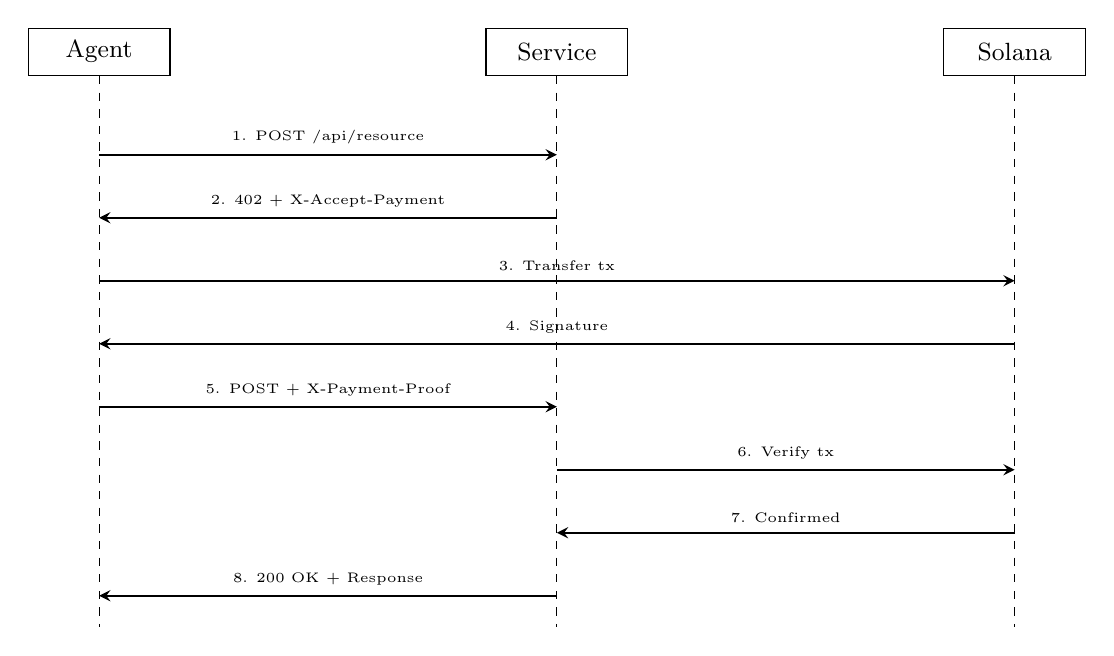
\begin{tikzpicture}[
    node distance=0.8cm,
    actor/.style={rectangle, draw, minimum width=1.8cm, minimum height=0.6cm, text centered, font=\small},
    msg/.style={->, >=stealth, thick},
    note/.style={font=\tiny, text width=3cm, align=center}
]
    % Actors
    \node[actor] (agent) {Agent};
    \node[actor, right=4cm of agent] (service) {Service};
    \node[actor, right=4cm of service] (solana) {Solana};
    
    % Lifelines
    \draw[dashed] (agent.south) -- ++(0,-7);
    \draw[dashed] (service.south) -- ++(0,-7);
    \draw[dashed] (solana.south) -- ++(0,-7);
    
    % Messages
    \draw[msg] ([yshift=-1cm]agent.south) -- ([yshift=-1cm]service.south) 
        node[midway, above, font=\tiny] {1. POST /api/resource};
    
    \draw[msg] ([yshift=-1.8cm]service.south) -- ([yshift=-1.8cm]agent.south) 
        node[midway, above, font=\tiny] {2. 402 + X-Accept-Payment};
    
    \draw[msg] ([yshift=-2.6cm]agent.south) -- ([yshift=-2.6cm]solana.south) 
        node[midway, above, font=\tiny] {3. Transfer tx};
    
    \draw[msg] ([yshift=-3.4cm]solana.south) -- ([yshift=-3.4cm]agent.south) 
        node[midway, above, font=\tiny] {4. Signature};
    
    \draw[msg] ([yshift=-4.2cm]agent.south) -- ([yshift=-4.2cm]service.south) 
        node[midway, above, font=\tiny] {5. POST + X-Payment-Proof};
    
    \draw[msg] ([yshift=-5cm]service.south) -- ([yshift=-5cm]solana.south) 
        node[midway, above, font=\tiny] {6. Verify tx};
    
    \draw[msg] ([yshift=-5.8cm]solana.south) -- ([yshift=-5.8cm]service.south) 
        node[midway, above, font=\tiny] {7. Confirmed};
    
    \draw[msg] ([yshift=-6.6cm]service.south) -- ([yshift=-6.6cm]agent.south) 
        node[midway, above, font=\tiny] {8. 200 OK + Response};
\end{tikzpicture}
\end{center}

\begin{center}
\small\textit{Figure 2: x402 Payment Flow. Agent receives 402, pays on-chain, then retries with proof.}
\end{center}

\subsection{Protocol Design}

\subsubsection{Payment Request}

When a service requires payment, it responds with HTTP 402 and an \texttt{X-Accept-Payment} header:

\begin{lstlisting}[language=HTTP,caption=HTTP 402 Payment Required Response]
HTTP/1.1 402 Payment Required
X-Accept-Payment: <base64-encoded-payment-request>
Content-Type: application/json

{
    "error": "payment_required",
    "message": "This endpoint requires payment"
}
\end{lstlisting}

The payment request (base64-decoded) contains:

\begin{lstlisting}[language=JSON,caption=Payment Request Structure]
{
    "version": "x0-v1",
    "recipient": "7xKXtg2CW87d97TXJSDpbD5jBkheTqA83TZRuJosgAsU",
    "amount": "1000000",
    "resource": "/api/v1/generate",
    "memo": "Text generation request",
    "network": "solana-mainnet",
    "escrow": {
        "use_escrow": false,
        "delivery_timeout": 3600,
        "auto_release_delay": 86400,
        "arbiter": null
    }
}
\end{lstlisting}

\subsubsection{Payment Proof}

After payment, the agent includes proof in subsequent requests:

\begin{lstlisting}[language=HTTP,caption=HTTP Request with Payment Proof]
POST /api/v1/generate HTTP/1.1
X-Payment-Proof: <base64-encoded-proof>
X-Payment-Version: x0-v1
Content-Type: application/json

{
    "prompt": "Generate a haiku about blockchain"
}
\end{lstlisting}

Payment proof contains:

\begin{lstlisting}[language=JSON,caption=Payment Proof Structure]
{
    "signature": "5VDx8F...",  // Transaction signature
    "slot": 123456789,
    "payer": "9xQeWv...",
    "timestamp": 1706400000,
    "network": "solana-mainnet"
}
\end{lstlisting}

\subsubsection{Verification}

The service verifies payment:

\begin{enumerate}
    \item Fetch transaction by signature
    \item Verify transaction succeeded
    \item Check recipient matches service wallet
    \item Check amount $\geq$ requested amount
    \item Verify timestamp within tolerance (±5 minutes)
    \item Check memo matches request (via SHA-256)
\end{enumerate}

\subsection{Security Properties}

\begin{theorem}[Payment Non-Repudiation]
A valid payment proof is unforgeable. An adversary cannot construct a proof without executing the on-chain transaction.
\end{theorem}

\begin{proof}
The proof contains transaction signature $\sigma = \texttt{Sign}(sk_A, tx)$. By existential unforgeability of Ed25519, an adversary cannot produce $\sigma'$ such that $\texttt{Verify}(pk_A, tx, \sigma') = 1$ without $sk_A$. On-chain verification ensures the transaction executed. \qed
\end{proof}

\section{Conditional Escrow (x0-escrow)}

\subsection{Design}

Escrow enables trustless payments for services with uncertain delivery.

\subsubsection{Escrow State Machine}

\begin{center}
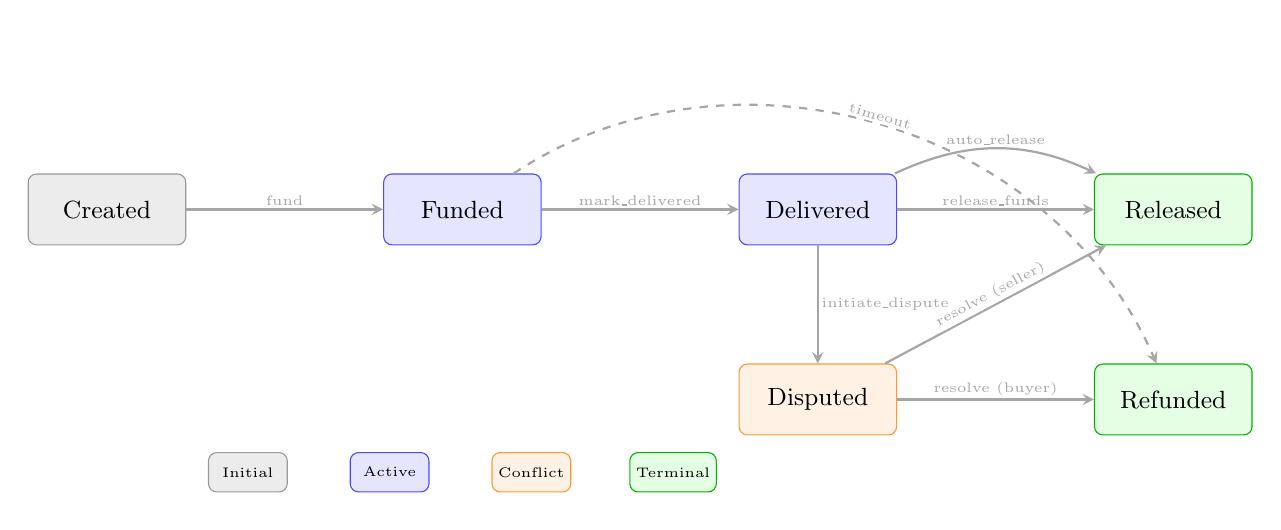
\begin{tikzpicture}[
    node distance=1.8cm and 2.5cm,
    % State styles with colors
    initial/.style={rectangle, rounded corners=3pt, draw=gray!80, fill=gray!15, 
        minimum width=2cm, minimum height=0.9cm, text centered, font=\small},
    active/.style={rectangle, rounded corners=3pt, draw=blue!70, fill=blue!10, 
        minimum width=2cm, minimum height=0.9cm, text centered, font=\small},
    conflict/.style={rectangle, rounded corners=3pt, draw=orange!80, fill=orange!10, 
        minimum width=2cm, minimum height=0.9cm, text centered, font=\small},
    terminal/.style={rectangle, rounded corners=3pt, draw=green!70!black, fill=green!10, 
        minimum width=2cm, minimum height=0.9cm, text centered, font=\small},
    % Arrow style
    arrow/.style={->, >=stealth, thick, color=gray!70},
    label/.style={font=\tiny, fill=white, inner sep=1pt}
]
    % States - arranged in logical flow
    \node[initial] (created) {Created};
    \node[active, right=of created] (funded) {Funded};
    \node[active, right=of funded] (delivered) {Delivered};
    \node[conflict, below=1.5cm of delivered] (disputed) {Disputed};
    \node[terminal, right=of delivered] (released) {Released};
    \node[terminal, below=1.5cm of released] (refunded) {Refunded};
    
    % Happy path (top row)
    \draw[arrow] (created) -- (funded) node[label, midway, above] {fund};
    \draw[arrow] (funded) -- (delivered) node[label, midway, above] {mark\_delivered};
    \draw[arrow] (delivered) -- (released) node[label, midway, above] {release\_funds};
    
    % Auto-release path
    \draw[arrow, bend left=25] (delivered) to node[label, above, sloped] {auto\_release} (released);
    
    % Dispute path
    \draw[arrow] (delivered) -- (disputed) node[label, midway, right] {initiate\_dispute};
    \draw[arrow] (disputed) -- (released) node[label, midway, above, sloped] {resolve (seller)};
    \draw[arrow] (disputed) -- (refunded) node[label, midway, above] {resolve (buyer)};
    
    % Timeout path
    \draw[arrow, dashed] (funded) to[bend left=50] node[label, above, sloped] {timeout} (refunded);
    
    % Legend
    \node[below=2.5cm of funded, font=\tiny] (legend) {
        \tikz{
            \node[initial, minimum width=1cm, minimum height=0.5cm, font=\tiny] at (0,0) {Initial};
            \node[active, minimum width=1cm, minimum height=0.5cm, font=\tiny] at (1.8,0) {Active};
            \node[conflict, minimum width=1cm, minimum height=0.5cm, font=\tiny] at (3.6,0) {Conflict};
            \node[terminal, minimum width=1cm, minimum height=0.5cm, font=\tiny] at (5.4,0) {Terminal};
        }
    };
\end{tikzpicture}
\end{center}

\begin{center}
\small\textit{Figure 3: Escrow State Machine. States are colored by type: gray (initial), blue (active), orange (conflict), green (terminal).}
\end{center}

\subsubsection{Escrow Account}

\begin{lstlisting}[language=Rust,caption=Escrow Account Structure]
#[account]
pub struct EscrowAccount {
    pub version: u8,                // Account version
    pub buyer: Pubkey,
    pub seller: Pubkey,
    pub arbiter: Option<Pubkey>,
    pub amount: u64,
    pub memo_hash: [u8; 32],
    pub state: EscrowState,
    pub timeout: i64,
    pub created_at: i64,
    pub delivery_proof: Option<[u8; 32]>,
    pub dispute_evidence: Option<[u8; 32]>,
    pub mint: Pubkey,
    pub token_decimals: u8,
    pub dispute_initiated_slot: u64, // MEDIUM-6: arbiter delay
    pub bump: u8,
}
\end{lstlisting}

\subsection{Key Operations}

\subsubsection{Create and Fund}

\begin{algorithm}
\caption{Create and Fund Escrow}
\begin{algorithmic}[1]
\Procedure{CreateEscrow}{$B, S, A, x, m, \tau$}
    \State \textbf{require} $B \neq S$
    \State \textbf{require} $3600 \leq \tau \leq 2592000$ \Comment{1h to 30d}
    \State $e \gets \texttt{EscrowPDA}(B, S, H(m))$
    \State $e.\texttt{timeout} \gets t_{\text{now}} + \tau$
    \State $e.\texttt{state} \gets \texttt{Created}$
    \State \Return $e$
\EndProcedure
\Procedure{FundEscrow}{$e, x$}
    \State \textbf{require} $e.\texttt{state} = \texttt{Created}$
    \State \textbf{require} $t_{\text{now}} < e.\texttt{timeout}$
    \State $\texttt{transfer}(B, e, x)$
    \State $e.\texttt{state} \gets \texttt{Funded}$
\EndProcedure
\end{algorithmic}
\end{algorithm}

\subsubsection{Delivery and Release}

\begin{algorithm}
\caption{Mark Delivered and Release Funds}
\begin{algorithmic}[1]
\Procedure{MarkDelivered}{$e, p$}
    \State \textbf{require} $\texttt{signer} = e.\texttt{seller}$
    \State \textbf{require} $e.\texttt{state} = \texttt{Funded}$
    \State $e.\texttt{delivery\_proof} \gets H(p)$
    \State $e.\texttt{state} \gets \texttt{Delivered}$
\EndProcedure
\Procedure{ReleaseFunds}{$e$}
    \State \textbf{require} $\texttt{signer} = e.\texttt{buyer}$
    \State \textbf{require} $e.\texttt{state} = \texttt{Delivered}$
    \State $e.\texttt{state} \gets \texttt{Released}$ \Comment{BEFORE transfer!}
    \State $\texttt{transfer}(e, e.\texttt{seller}, e.\texttt{amount})$
    \State $\texttt{UpdateReputation}(e.\texttt{seller}, \texttt{Success})$ \Comment{Optional CPI}
\EndProcedure
\end{algorithmic}
\end{algorithm}

\subsubsection{Auto-Release}

After delivery, if buyer doesn't dispute within timeout, seller can claim:

\begin{algorithm}
\caption{Auto-Release After Timeout}
\begin{algorithmic}[1]
\Procedure{ClaimAutoRelease}{$e$}
    \State \textbf{require} $\texttt{signer} = e.\texttt{seller}$
    \State \textbf{require} $e.\texttt{state} = \texttt{Delivered}$
    \State \textbf{require} $t_{\text{now}} > e.\texttt{timeout}$
    \State $e.\texttt{state} \gets \texttt{Released}$
    \State $\texttt{transfer}(e, e.\texttt{seller}, e.\texttt{amount})$
    \State $\texttt{UpdateReputation}(e.\texttt{seller}, \texttt{Success})$
\EndProcedure
\end{algorithmic}
\end{algorithm}

\subsubsection{Dispute Resolution}

\begin{algorithm}
\caption{Initiate and Resolve Dispute}
\begin{algorithmic}[1]
\Procedure{InitiateDispute}{$e, d$}
    \State \textbf{require} $\texttt{signer} \in \{e.\texttt{buyer}, e.\texttt{seller}\}$
    \State \textbf{require} $e.\texttt{state} = \texttt{Delivered}$
    \State $e.\texttt{dispute\_evidence} \gets H(d)$
    \State $e.\texttt{dispute\_initiated\_slot} \gets \texttt{current\_slot}$
    \State $e.\texttt{state} \gets \texttt{Disputed}$
    \State $\texttt{UpdateReputation}(e.\texttt{seller}, \texttt{Dispute})$
\EndProcedure
\Procedure{ResolveDispute}{$e, \texttt{release\_to\_seller}$}
    \State \textbf{require} $\texttt{signer} = e.\texttt{arbiter}$
    \State \textbf{require} $e.\texttt{state} = \texttt{Disputed}$
    \State \textbf{require} $\texttt{current\_slot} \geq e.\texttt{dispute\_initiated\_slot} + \Delta$
    \State \Comment{$\Delta = 216000$ slots $\approx$ 24 hours}
    \If{$\texttt{release\_to\_seller}$}
        \State $e.\texttt{state} \gets \texttt{Released}$
        \State $\texttt{transfer}(e, e.\texttt{seller}, e.\texttt{amount})$
        \State $\texttt{UpdateReputation}(e.\texttt{seller}, \texttt{ResolutionFavor})$
    \Else
        \State $e.\texttt{state} \gets \texttt{Refunded}$
        \State $\texttt{transfer}(e, e.\texttt{buyer}, e.\texttt{amount})$
    \EndIf
\EndProcedure
\end{algorithmic}
\end{algorithm}

\subsection{Security Analysis}

\begin{theorem}[Escrow Safety]
An escrow satisfies:
\begin{enumerate}
    \item \textbf{Atomicity}: Funds are either fully released or refunded, never partially
    \item \textbf{Liveness}: Funds are never permanently locked
    \item \textbf{Fairness}: Either party can initiate dispute; arbiter is neutral
\end{enumerate}
\end{theorem}

\begin{proof}
\textbf{Atomicity}: State transitions are atomic. The \texttt{Released} and \texttt{Refunded} states are terminal.

\textbf{Liveness}: Three exit paths exist:
\begin{itemize}
    \item Buyer releases after delivery
    \item Seller claims auto-release after timeout
    \item Arbiter resolves dispute
\end{itemize}
At least one path is always available after delivery or timeout.

\textbf{Fairness}: Either party can initiate dispute. Arbiter resolution requires evidence from both parties and a 24-hour delay. \qed
\end{proof}

\section{Reputation Oracle (x0-reputation)}

\subsection{Design Goals}

\begin{enumerate}
    \item \textbf{Transparency}: All reputation data on-chain
    \item \textbf{Temporal Decay}: Old successes shouldn't dominate forever
    \item \textbf{Sybil Resistance}: New agents don't get perfect scores
    \item \textbf{Nuanced Scoring}: Distinguish success, failure, disputes, resolutions
\end{enumerate}

\subsection{Reputation Account}

\begin{lstlisting}[language=Rust,caption=Reputation Account Structure]
#[account]
pub struct AgentReputation {
    pub version: u8,                   // Account version (v2)
    pub agent_id: Pubkey,
    pub total_transactions: u64,
    pub successful_transactions: u64,
    pub disputed_transactions: u64,
    pub resolved_in_favor: u64,
    pub failed_transactions: u64,      // Policy rejections
    pub average_response_time_ms: u32,
    pub cumulative_response_time_ms: u64,
    pub last_updated: i64,
    pub last_decay_applied: i64,
    pub bump: u8,
}
\end{lstlisting}

\subsection{Reputation Score Calculation}

\begin{definition}[Reputation Score]
The reputation score $S \in [0, 1]$ is computed as:
\begin{align}
S &= 0.60 \cdot S_{\text{success}} + 0.15 \cdot S_{\text{resolution}} \nonumber \\
&\quad + 0.10 \cdot (1 - R_{\text{dispute}}) + 0.15 \cdot (1 - R_{\text{failure}})
\end{align}
where:
\begin{align}
S_{\text{success}} &= \frac{n_{\text{success}}}{n_{\text{total}}} \\
S_{\text{resolution}} &= \begin{cases}
\frac{n_{\text{resolved}}}{n_{\text{disputed}}} & n_{\text{disputed}} > 0 \\
0.5 & n_{\text{disputed}} = 0 \land n_{\text{total}} < 10 \\
1.0 & n_{\text{disputed}} = 0 \land n_{\text{total}} \geq 10
\end{cases} \\
R_{\text{dispute}} &= \frac{n_{\text{disputed}}}{n_{\text{total}}} \\
R_{\text{failure}} &= \frac{n_{\text{failed}}}{n_{\text{total}}}
\end{align}
\end{definition}

\begin{remark}
The neutral resolution score (0.5) for new agents prevents Sybil attacks where attackers create new identities to get perfect scores.
\end{remark}

\begin{example}[Reputation Score Calculation]
Consider an agent with the following transaction history:
\begin{itemize}
    \item Total transactions: $n_{\text{total}} = 100$
    \item Successful: $n_{\text{success}} = 90$
    \item Disputed: $n_{\text{disputed}} = 5$
    \item Resolved in favor: $n_{\text{resolved}} = 3$
    \item Failed (policy rejections): $n_{\text{failed}} = 2$
\end{itemize}

Computing component scores:
\begin{align*}
S_{\text{success}} &= \frac{90}{100} = 0.90 \\
S_{\text{resolution}} &= \frac{3}{5} = 0.60 \quad (\text{since } n_{\text{disputed}} > 0) \\
R_{\text{dispute}} &= \frac{5}{100} = 0.05 \\
R_{\text{failure}} &= \frac{2}{100} = 0.02
\end{align*}

Final reputation score:
\begin{align*}
S &= 0.60(0.90) + 0.15(0.60) + 0.10(1 - 0.05) + 0.15(1 - 0.02) \\
&= 0.540 + 0.090 + 0.095 + 0.147 \\
&= \mathbf{0.872}
\end{align*}

This agent has a strong reputation (87.2\%), with room for improvement in dispute resolution.
\end{example}

\subsection{Temporal Decay}

\begin{definition}[Exponential Decay]
Monthly decay applies to successful transactions:
\begin{equation}
n_{\text{success}}^{(t+1)} = n_{\text{success}}^{(t)} \cdot (1 - \alpha)
\end{equation}
where $\alpha = 0.01$ (1\% monthly decay) and $t$ is measured in months.
\end{definition}

For $m$ months:
\begin{equation}
n_{\text{success}}^{(t+m)} = n_{\text{success}}^{(t)} \cdot (0.99)^m
\end{equation}

\begin{proposition}[Half-Life]
The half-life of reputation is:
\begin{equation}
t_{1/2} = \frac{\ln 2}{\ln(1/0.99)} \approx 69 \text{ months}
\end{equation}
\end{proposition}

\begin{algorithm}
\caption{Apply Reputation Decay}
\begin{algorithmic}[1]
\Procedure{ApplyDecay}{$r$}
    \State $m \gets \lfloor (t_{\text{now}} - r.\texttt{last\_decay\_applied}) / 2592000 \rfloor$
    \If{$m > 0$}
        \State $d_{\text{mult}} \gets 99^{\min(m, 12)}$ \Comment{Cap at 12 months}
        \State $d_{\text{div}} \gets 100^{\min(m, 12)}$
        \State $r.\texttt{successful\_transactions} \gets r.\texttt{successful\_transactions} \cdot d_{\text{mult}} / d_{\text{div}}$
        \State $r.\texttt{last\_decay\_applied} \gets t_{\text{now}}$
    \EndIf
\EndProcedure
\end{algorithmic}
\end{algorithm}

\subsection{Authorization Model}

\begin{definition}[Authorized Callers]
Reputation updates can only be called by:
\begin{itemize}
    \item \textbf{Escrow program}: Records success/dispute/resolution
    \item \textbf{Guard program}: Records policy failures
    \item \textbf{Policy owner}: Self-reported off-chain transactions
\end{itemize}
\end{definition}

\begin{theorem}[Reputation Integrity]
An adversary cannot artificially inflate reputation without:
\begin{enumerate}
    \item Completing escrow transactions (requires payment)
    \item Winning disputes (requires arbiter approval)
    \item Controlling policy owner key (equivalent to ownership)
\end{enumerate}
\end{theorem}

\section{Agent Discovery (x0-registry)}

\subsection{Registry Entry}

\begin{lstlisting}[language=Rust,caption=Registry Entry Structure]
#[account]
pub struct AgentRegistry {
    pub version: u8,                   // Account version
    pub agent_id: Pubkey,              // Policy PDA (primary ID)
    pub owner: Pubkey,                 // Owner who can update
    pub endpoint: String,              // Service URL (max 256 chars)
    pub capabilities: Vec<Capability>, // Max 10 capabilities
    pub price_oracle: Option<Pubkey>,  // Optional pricing oracle
    pub reputation_pda: Pubkey,        // Linked reputation account
    pub last_updated: i64,
    pub is_active: bool,
    pub bump: u8,
}

pub struct Capability {
    pub capability_type: String,       // Max 64 chars
    pub metadata: String,              // JSON metadata (max 256 chars)
}
\end{lstlisting}

The \texttt{Capability} struct uses a JSON \texttt{metadata} field to encode pricing, versioning, and service-specific parameters (see Section~\ref{sec:capability-metadata}), avoiding rigid on-chain schema constraints.

\subsection{Discovery Algorithm}

\begin{algorithm}
\caption{Find Agents by Capability}
\begin{algorithmic}[1]
\Procedure{FindAgents}{$\texttt{cap\_type}$}
    \State $A \gets \{\}$ \Comment{Set of matching agents}
    \For{$e \in \texttt{GetProgramAccounts}(\texttt{registry\_program})$}
        \If{$\texttt{cap\_type} \in e.\texttt{capabilities} \land e.\texttt{is\_active}$}
            \State $s \gets \texttt{FetchReputation}(e.\texttt{reputation\_pda})$
            \State $A \gets A \cup \{(e, s)\}$
        \EndIf
    \EndFor
    \State \Return $\texttt{SortByScore}(A)$
\EndProcedure
\end{algorithmic}
\end{algorithm}

\subsection{Capability Metadata}\label{sec:capability-metadata}

Capabilities use JSON metadata:

\begin{lstlisting}[language=JSON,caption=Capability Metadata Example]
{
    "type": "text-generation",
    "models": ["gpt-4", "claude-3"],
    "pricing": {
        "per_token": 0.00001,
        "minimum": 0.01
    },
    "rate_limit": {
        "requests_per_minute": 60,
        "burst": 10
    },
    "api_version": "v1"
}
\end{lstlisting}

\section{USDC Wrapper (x0-wrapper)}

\subsection{Problem Statement}

Direct USDC usage has limitations:
\begin{enumerate}
    \item No transfer hook support on standard USDC
    \item Different token programs (SPL vs Token-2022)
    \item Protocol fees require wrapper
\end{enumerate}

\subsection{Design}

x0-USD is a 1:1 USDC-backed Token-2022 token with:
\begin{itemize}
    \item Transfer hook pointing to x0-guard
    \item 0.8\% transfer fee (configurable via \texttt{PROTOCOL\_FEE\_BASIS\_POINTS} constant, default 80 bps)
    \item Configurable redemption fee (default 0.8\%, set via \texttt{WRAPPER\_REDEMPTION\_FEE\_BPS})
\end{itemize}

\subsubsection{State Accounts}

The wrapper maintains two on-chain accounts for configuration and operational metrics:

\begin{lstlisting}[language=Rust,caption=Wrapper Configuration Account]
#[account]
pub struct WrapperConfig {
    pub admin: Pubkey,                 // Admin key (should be multisig)
    pub pending_admin: Option<Pubkey>, // Two-step admin transfer
    pub usdc_mint: Pubkey,             // Underlying USDC mint
    pub wrapper_mint: Pubkey,          // x0-USD mint
    pub reserve_account: Pubkey,       // USDC reserve token account
    pub redemption_fee_bps: u16,       // Fee in basis points
    pub is_paused: bool,               // Emergency pause flag
    pub bump: u8,
}
\end{lstlisting}

\begin{lstlisting}[language=Rust,caption=Wrapper Statistics Account]
#[account]
pub struct WrapperStats {
    pub reserve_usdc_balance: u64,     // Current USDC in reserve
    pub outstanding_wrapper_supply: u64, // Outstanding x0-USD supply
    pub total_deposits: u64,           // All-time deposits
    pub total_redemptions: u64,        // All-time redemptions
    pub total_fees_collected: u64,     // All-time fees
    pub daily_redemption_volume: u64,  // Resets every 24h
    pub daily_redemption_reset_timestamp: i64,
    pub last_updated: i64,
    pub bump: u8,
}
\end{lstlisting}

The reserve ratio $\rho$ can be computed directly from \texttt{WrapperStats}:
\begin{equation}
\rho = \frac{\texttt{reserve\_usdc\_balance}}{\texttt{outstanding\_wrapper\_supply}}
\end{equation}

\subsubsection{Reserve Invariant}

\begin{definition}[Reserve Invariant]
At all times, the following must hold:
\begin{equation}
R_{\text{USDC}} \geq S_{\text{x0-USD}}
\end{equation}
where $R_{\text{USDC}}$ is USDC reserve and $S_{\text{x0-USD}}$ is outstanding x0-USD supply.
\end{definition}

\begin{theorem}[Invariant Preservation]
The reserve invariant is preserved under all operations.
\end{theorem}

\begin{proof}
We prove by cases:

\textbf{Deposit}: User deposits $x$ USDC, receives $x$ x0-USD.
\begin{equation}
R' = R + x, \quad S' = S + x \implies R' - S' = R - S \geq 0
\end{equation}

\textbf{Redemption}: User burns $x$ x0-USD, receives $x - f$ USDC (fee $f$).
\begin{equation}
R' = R - (x - f), \quad S' = S - x
\end{equation}
\begin{equation}
R' - S' = R - x + f - S + x = R - S + f \geq R - S \geq 0
\end{equation}

The fee increases the reserve ratio. \qed
\end{proof}

\subsection{Governance}

\subsubsection{Timelock}

All admin operations require 48-hour timelock. Each pending action is stored in a PDA:

\begin{lstlisting}[language=Rust,caption=Timelocked Admin Action]
#[account]
pub struct AdminAction {
    pub action_type: AdminActionType,  // SetFeeRate | SetPaused | EmergencyWithdraw | TransferAdmin
    pub scheduled_timestamp: i64,      // Earliest execution time
    pub new_value: u64,                // Interpretation depends on action_type
    pub new_admin: Pubkey,             // For TransferAdmin actions
    pub destination: Pubkey,           // For EmergencyWithdraw
    pub executed: bool,
    pub cancelled: bool,
    pub bump: u8,
}
\end{lstlisting}

An action is executable if and only if $t_{\text{now}} \geq \texttt{scheduled\_timestamp}$ and $\neg \texttt{executed} \land \neg \texttt{cancelled}$.

\begin{algorithm}
\caption{Timelock Pattern}
\begin{algorithmic}[1]
\Procedure{ScheduleAction}{$a, v, t$}
    \State $\texttt{action\_pda} \gets \texttt{CreateActionPDA}(a, \texttt{nonce})$
    \State $\texttt{action\_pda.type} \gets a$
    \State $\texttt{action\_pda.value} \gets v$
    \State $\texttt{action\_pda.scheduled\_time} \gets t + 172800$ \Comment{48h}
\EndProcedure
\Procedure{ExecuteAction}{$\texttt{action\_pda}$}
    \State \textbf{require} $t_{\text{now}} \geq \texttt{action\_pda.scheduled\_time}$
    \State \textbf{require} $\neg \texttt{action\_pda.executed}$
    \State \textbf{require} $\neg \texttt{action\_pda.cancelled}$
    \State $\texttt{ApplyAction}(\texttt{action\_pda.type}, \texttt{action\_pda.value})$
    \State $\texttt{action\_pda.executed} \gets \texttt{true}$
\EndProcedure
\end{algorithmic}
\end{algorithm}

\subsubsection{Emergency Pause}

Emergency pause is the \textbf{only} operation bypassing timelock:
\begin{itemize}
    \item Can only \textbf{pause}, never unpause
    \item Unpausing requires standard timelock
    \item Prevents rapid pause/unpause attacks
\end{itemize}

\subsection{Reserve Ratio Monitoring}

\begin{definition}[Reserve Ratio]
\begin{equation}
\rho = \frac{R_{\text{USDC}}}{S_{\text{x0-USD}}}
\end{equation}
\end{definition}

Alert levels:
\begin{itemize}
    \item $\rho < 1.01$: Warning alert
    \item $\rho < 1.00$: Critical alert (undercollateralized)
\end{itemize}

\section{Human-in-the-Loop (Blinks)}

\subsection{Problem Statement}

Full automation is dangerous for:
\begin{enumerate}
    \item Transfers exceeding daily limit
    \item Recipients not on whitelist
    \item Unusually large transactions
\end{enumerate}

\subsection{Blink Design}

A \textbf{Blink} is a Solana Action requesting human approval.

\subsubsection{Generation}

When guard rejects a transfer due to limits, it can:
\begin{enumerate}
    \item Generate Blink ID: $b = H(\texttt{policy} \parallel R \parallel x \parallel t)[0..16]$
    \item Emit \texttt{BlinkGenerated} event with:
    \begin{itemize}
        \item Blink ID
        \item Requested amount
        \item Recipient
        \item Expiration (15 minutes)
    \end{itemize}
    \item Charge fee (0.001 SOL) to prevent spam
\end{enumerate}

\subsubsection{Rate Limiting}

\begin{definition}[Blink Rate Limit]
Maximum 3 Blinks per hour per policy.
\end{definition}

\begin{algorithm}
\caption{Blink Rate Limit Check}
\begin{algorithmic}[1]
\Procedure{CheckBlinkRateLimit}{$p, t$}
    \State $h_{\text{current}} \gets \lfloor t / 3600 \rfloor$
    \State $h_{\text{window}} \gets \lfloor p.\texttt{blink\_hour\_start} / 3600 \rfloor$
    \If{$h_{\text{current}} \neq h_{\text{window}}$}
        \State $p.\texttt{blink\_hour\_start} \gets t$
        \State $p.\texttt{blinks\_this\_hour} \gets 0$
    \EndIf
    \If{$p.\texttt{blinks\_this\_hour} \geq 3$}
        \State \Return \texttt{false}
    \EndIf
    \State $p.\texttt{blinks\_this\_hour} \gets p.\texttt{blinks\_this\_hour} + 1$
    \State \Return \texttt{true}
\EndProcedure
\end{algorithmic}
\end{algorithm}

\subsubsection{Approval}

Owner approves via:
\begin{enumerate}
    \item Viewing Blink details (QR code, web interface, wallet)
    \item Signing approval transaction
    \item Temporarily raising limit or whitelisting recipient
\end{enumerate}

\section{Economic Model}

\subsection{Fee Structure}

\begin{table}[ht!]
\centering
\begin{tabular}{|l|l|l|}
\hline
\textbf{Operation} & \textbf{Fee} & \textbf{Recipient} \\
\hline
Transfer (x0-USD) & 0.8\% & Protocol treasury \\
Registry listing & 0.1 SOL & Protocol treasury \\
Blink generation & 0.001 SOL & Protocol treasury \\
Wrapper redemption & 0.8\% (configurable) & Wrapper reserve \\
\hline
\end{tabular}
\caption{Protocol Fee Schedule}
\end{table}

\subsection{Fee Collection}

Transfer fees are collected via Token-2022's TransferFee extension:

\begin{algorithm}
\caption{Fee Harvesting}
\begin{algorithmic}[1]
\Procedure{HarvestFees}{$\texttt{mint}, \texttt{accounts}$}
    \For{$a \in \texttt{accounts}$}
        \State $f \gets \texttt{GetWithheldAmount}(a)$
        \State $\texttt{TransferWithheldToMint}(a, f)$
    \EndFor
    \State $F \gets \sum_a f$
    \State $\texttt{WithdrawWithheldFromMint}(\texttt{mint}, \texttt{treasury}, F)$
\EndProcedure
\end{algorithmic}
\end{algorithm}

\subsection{Token Economics}

\subsubsection{x0-USD Supply Dynamics}

\begin{align}
\frac{dS}{dt} &= D(t) - R(t) \\
\frac{dR_{\text{USDC}}}{dt} &= D(t) - R(t) + f \cdot R(t)
\end{align}

where:
\begin{itemize}
    \item $S(t)$ = x0-USD supply
    \item $R_{\text{USDC}}(t)$ = USDC reserve
    \item $D(t)$ = Deposit rate
    \item $R(t)$ = Redemption rate (before fees)
    \item $f$ = Redemption fee rate
\end{itemize}

Reserve ratio evolution:
\begin{equation}
\rho(t) = \frac{R_{\text{USDC}}(t)}{S(t)} = 1 + \int_0^t \frac{f \cdot R(\tau)}{S(\tau)} d\tau
\end{equation}

The reserve ratio increases over time due to fees.

\section{Zero-Knowledge Proof Verification (x0-zk-verifier)}

\subsection{Problem Statement}

Token-2022's Confidential Transfer extension encrypts token balances and transfer amounts using twisted ElGamal encryption over the Ristretto255 curve. To ensure that encrypted operations preserve token invariants (e.g., non-negative balances, valid public keys), the protocol requires zero-knowledge proofs that attest to the correctness of ciphertext operations without revealing plaintext values.

The challenge is two-fold:
\begin{enumerate}
    \item \textbf{Client-side proof generation}: Proofs must be generated off-chain where the user holds the ElGamal secret key, using Groth16 proving circuits from \texttt{solana-zk-token-sdk}.
    \item \textbf{On-chain proof verification}: Proofs must be verified on-chain and the verification result stored in a state account that Token-2022 can reference during confidential transfer execution.
\end{enumerate}

\subsection{Cryptographic Foundations}

\subsubsection{Twisted ElGamal Encryption}

Token-2022 uses a \emph{twisted} variant of ElGamal encryption over the Ristretto255 group, which provides both encryption and efficient homomorphic addition:

\begin{definition}[Twisted ElGamal Encryption]
For a public key $P = s \cdot G$ where $s$ is the secret scalar and $G$ is the Ristretto255 basepoint:
\begin{align}
\texttt{Encrypt}(P, v) &= (r \cdot G, \; r \cdot P + v \cdot H) \\
\texttt{Decrypt}(s, (C_1, C_2)) &= C_2 - s \cdot C_1 = v \cdot H
\end{align}
where $r \stackrel{\$}{\leftarrow} \mathbb{Z}_q$ is a random scalar, $H$ is a second generator, and $v$ is the plaintext value. Decryption recovers $v \cdot H$, from which $v$ is obtained via brute-force discrete log (feasible for $v < 2^{48}$).
\end{definition}

\subsubsection{Groth16 Proof System}

The protocol uses Groth16~\cite{groth16} for succinct non-interactive zero-knowledge proofs:

\begin{definition}[Groth16 Proof]
A Groth16 proof $\pi = (A, B, C) \in \mathbb{G}_1 \times \mathbb{G}_2 \times \mathbb{G}_1$ proves knowledge of a witness $w$ satisfying a rank-1 constraint system $R(x, w) = 1$, where $x$ is the public input. The proof satisfies:
\begin{itemize}
    \item \textbf{Completeness}: An honest prover always produces a valid proof
    \item \textbf{Soundness}: No efficient adversary can produce a valid proof for a false statement
    \item \textbf{Zero-knowledge}: The proof reveals nothing about $w$ beyond $R(x, w) = 1$
\end{itemize}
Proof size is constant: 192 bytes regardless of circuit complexity.
\end{definition}

\subsection{Proof Types}

The verifier supports four proof types corresponding to Token-2022 confidential transfer operations:

\subsubsection{PubkeyValidityProof}

Proves that a given 32-byte value is a valid ElGamal public key (i.e., a point on the Ristretto255 curve that was correctly derived from a secret key).

\begin{equation}
\text{Prove}: \exists \; s \in \mathbb{Z}_q \text{ such that } P = s \cdot G
\end{equation}

Required when configuring a token account for confidential transfers. Proof data is 64 bytes.

\subsubsection{ZeroBalanceProof}

Proves that an ElGamal ciphertext encrypts the value zero, required for account closure:

\begin{equation}
\text{Prove}: (C_1, C_2) = \texttt{Encrypt}(P, 0) \implies C_2 = r \cdot P
\end{equation}

Proof data is 96 bytes.

\subsubsection{WithdrawProof}

Proves that a withdrawal of amount $a$ from an encrypted balance $B$ is valid:

\begin{equation}
\text{Prove}: \texttt{Decrypt}(s, B) = v \geq a \;\land\; B' = B - \texttt{Encrypt}(P, a)
\end{equation}

where $v$ is the current balance and $B'$ is the new encrypted balance. This ensures the account has sufficient funds without revealing either the balance or the withdrawal amount on-chain. Proof data is 160 bytes.

\subsubsection{TransferProof}

Proves the correctness of a confidential transfer between two accounts:

\begin{equation}
\text{Prove}: \texttt{Decrypt}(s_{\text{src}}, B_{\text{src}}) \geq a \;\land\; B'_{\text{src}} = B_{\text{src}} - \texttt{Encrypt}(P_{\text{src}}, a) \;\land\; \Delta_{\text{dst}} = \texttt{Encrypt}(P_{\text{dst}}, a)
\end{equation}

This is the most complex proof, attesting simultaneously that the sender has sufficient balance, the sender's balance is correctly decremented, and the recipient's balance increment is correctly encrypted under the recipient's public key.

\subsection{Architecture}

\subsubsection{Proof Context Account}

Successful verification creates a \texttt{ProofContext} PDA that stores the verification result:

\begin{lstlisting}[language=Rust,caption=Proof Context State Account]
#[account]
pub struct ProofContext {
    pub version: u8,
    pub proof_type: ProofType,         // PubkeyValidity | Withdraw | ZeroBalance | Transfer
    pub verified: bool,
    pub owner: Pubkey,                 // Account owner who can use this proof
    pub verified_at: i64,              // Unix timestamp
    pub amount: Option<u64>,           // For Withdraw/Transfer proofs
    pub recipient: Option<Pubkey>,     // For Transfer proofs
    pub elgamal_pubkey: Option<[u8; 32]>, // For PubkeyValidity proofs
    pub mint: Pubkey,                  // Token mint this proof is for
    pub token_account: Pubkey,         // Token account this proof is for
    pub bump: u8,
}
\end{lstlisting}

\subsubsection{Proof Freshness}

To prevent replay attacks, proof contexts enforce a temporal validity window:

\begin{definition}[Proof Freshness]
A proof context $C$ is \emph{fresh} at time $t$ if and only if:
\begin{equation}
t - C.\texttt{verified\_at} < \Delta_{\text{proof}} = 300 \text{ seconds}
\end{equation}
\end{definition}

The 5-minute window provides sufficient time for transaction construction and submission while limiting the replay window.

\subsubsection{Amount Bounds}

All confidential amounts are bounded:
\begin{equation}
0 \leq a \leq 2^{48} - 1 = 281{,}474{,}976{,}710{,}655
\end{equation}

This constraint arises from the brute-force discrete log required during ElGamal decryption. The \texttt{solana-zk-token-sdk} uses a precomputed lookup table for values up to $2^{16}$, combined with baby-step-giant-step for the remaining $2^{32}$ range.

\subsection{Off-Chain Proof Generation (x0-zk-proofs)}

The \texttt{x0-zk-proofs} crate is a Rust library compiled to WebAssembly via \texttt{wasm-pack}, providing client-side proof generation for the TypeScript SDK:

\begin{lstlisting}[language=Rust,caption=x0-zk-proofs WASM Interface]
#[wasm_bindgen]
pub fn generate_pubkey_validity_proof(
    keypair_bytes: &[u8]        // 64-byte ElGamalKeypair
) -> Result<Vec<u8>, JsValue>;  // 64-byte PubkeyValidityData

#[wasm_bindgen]
pub fn generate_zero_balance_proof(
    keypair_bytes: &[u8]        // 64-byte ElGamalKeypair
) -> Result<Vec<u8>, JsValue>;  // 96-byte ZeroBalanceProofData

#[wasm_bindgen]
pub fn generate_withdraw_proof(
    keypair_bytes: &[u8],       // 64-byte ElGamalKeypair
    current_balance: u64,       // Current decrypted balance
    withdraw_amount: u64        // Amount to withdraw
) -> Result<Vec<u8>, JsValue>;  // 160-byte WithdrawData
\end{lstlisting}

The WASM module internally uses:
\begin{itemize}
    \item \texttt{solana-zk-token-sdk v1.18.22} for Groth16 circuit construction and proving
    \item \texttt{ElGamalKeypair} reconstruction from 64-byte serialized form
    \item \texttt{bytemuck} for zero-copy POD serialization of proof data
    \item Authenticated encryption (AE) ciphertexts for decryptable balance hints
\end{itemize}

\subsection{Verification Flow}

The end-to-end flow for a confidential withdrawal is:

\begin{algorithm}
\caption{Confidential Withdrawal with ZK Proof}
\begin{algorithmic}[1]
\Procedure{ConfidentialWithdraw}{$\texttt{keypair}, b, a$}
    \State \textbf{require} $a \leq b$ \Comment{Client-side: sufficient balance}
    \State \textbf{require} $a \leq 2^{48} - 1$ \Comment{Client-side: amount bound}
    \State $\pi \gets \texttt{x0\_zk\_proofs::generate\_withdraw\_proof}(\texttt{keypair}, b, a)$
    \State \textbf{send} $\texttt{x0\_zk\_verifier::verify\_withdraw}(\pi, a, \texttt{new\_ae\_balance})$
    \State $C \gets \texttt{ProofContext PDA}$ \Comment{On-chain: created after verification}
    \State \textbf{require} $C.\texttt{verified} = \texttt{true}$ \Comment{On-chain check}
    \State \textbf{send} $\texttt{Token-2022::confidential\_withdraw}(a, C)$
\EndProcedure
\end{algorithmic}
\end{algorithm}

\subsection{Security Properties}

\begin{theorem}[Balance Confidentiality]
An adversary observing the blockchain cannot determine any agent's confidential balance, even given all historic proof contexts and ciphertexts.
\end{theorem}

\begin{proof}
Token balances are encrypted under twisted ElGamal with semantic security. Proof contexts store only the verification result, proof type, and amount (for withdrawals), but the \emph{remaining balance} is revealed only via AE ciphertext decryptable solely by the account holder. The Groth16 zero-knowledge property ensures proofs reveal nothing beyond the statement's truth. \qed
\end{proof}

\begin{theorem}[Proof Unforgeability]
No computationally bounded adversary can produce a valid proof for a false statement (e.g., withdrawing more than the encrypted balance).
\end{theorem}

\begin{proof}
Follows from the knowledge-soundness of Groth16 under the $q$-type knowledge-of-exponent assumption in bilinear groups. The verifier re-derives the check via \texttt{solana-zk-token-sdk}'s \texttt{verify()}, which evaluates the Groth16 pairing equation. \qed
\end{proof}

\section{Security Analysis}

\subsection{Threat Model}

We consider the following adversaries:

\begin{enumerate}
    \item \textbf{Compromised Agent}: Attacker obtains $sk_A$
    \item \textbf{Malicious Service}: Service provider attempts fraud
    \item \textbf{Malicious Agent}: Agent attempts reputation manipulation
    \item \textbf{Wrapper Attack}: Attacker attempts reserve drain
    \item \textbf{Bridge Attack}: Attacker attempts cross-chain fund extraction (see Section~14.10 for bridge-specific analysis)
\end{enumerate}

\subsection{Attack Scenarios and Mitigations}

\subsubsection{Compromised Agent Key}

\textbf{Attack}: Adversary steals $sk_A$, attempts unlimited spending.

\textbf{Mitigation}: 
\begin{itemize}
    \item Rolling window limits spending to $L$ per 24 hours
    \item Owner can revoke via \texttt{revoke\_agent\_authority}
    \item Maximum loss bounded by $L + x_{\text{max}}$ where $x_{\text{max}}$ is max transaction size
\end{itemize}

\subsubsection{Sybil Attack on Reputation}

\textbf{Attack}: Adversary creates multiple identities to appear trustworthy.

\textbf{Mitigation}:
\begin{itemize}
    \item Registry listing costs 0.1 SOL
    \item New agents get neutral (0.5) resolution score, not perfect
    \item Temporal decay prevents dormant identities
\end{itemize}

Cost for 100 Sybil identities: $100 \times 0.1 = 10$ SOL $\approx \$1000$ (at \$100/SOL).

\subsubsection{Escrow Griefing}

\textbf{Attack}: Malicious buyer creates many escrows, ties up seller funds.

\textbf{Mitigation}:
\begin{itemize}
    \item Escrow creation is permissionless but buyer must fund
    \item Sellers can set minimum transaction amounts
    \item Reputation tracking penalizes frivolous disputes
\end{itemize}

\subsubsection{Wrapper Reserve Drain}

\textbf{Attack}: Exploit bug to withdraw USDC without burning x0-USD.

\textbf{Mitigation}:
\begin{itemize}
    \item Reserve invariant checked before every redemption
    \item State updated before transfer (reentrancy protection)
    \item Admin operations timelocked (48h notice)
    \item Emergency pause available
\end{itemize}

\subsubsection{Transfer Hook Configuration Attack}

\textbf{Attack}: Unauthorized party front-runs transfer hook initialization for a mint, potentially misconfiguring the extra account metas or consuming the PDA address.

\textbf{Mitigation}:
\begin{itemize}
    \item Only the Token-2022 mint authority can initialize extra account metas
    \item Re-initialization is blocked after first valid configuration
    \item Extra account metas configuration is deterministic (not caller-supplied)
    \item Mint authority verification uses \texttt{StateWithExtensions} for robust parsing
\end{itemize}

\textbf{Impact}: Even though the extra metas configuration is hardcoded in the program, preventing unauthorized initialization eliminates a griefing vector where an attacker could pay the rent and claim the PDA before the legitimate mint authority initializes it.

\subsection{Formal Verification}

\subsubsection{Spend Limit Invariant}

\begin{theorem}[Daily Spend Limit]
For all execution traces, if policy has daily limit $L$:
\begin{equation}
\forall t: \sum_{i: t_i > t - 86400} x_i \leq L
\end{equation}
\end{theorem}

\begin{proof}
Proven in Section 3.4. \qed
\end{proof}

\subsubsection{Reserve Invariant}

\begin{theorem}[Wrapper Reserve Invariant]
For all execution traces:
\begin{equation}
\forall t: R_{\text{USDC}}(t) \geq S_{\text{x0-USD}}(t)
\end{equation}
\end{theorem}

\begin{proof}
Proven in Section 7.2. \qed
\end{proof}

\section{Performance Analysis}

\subsection{Computational Complexity}

\begin{table}[ht!]
\centering
\begin{tabular}{|l|l|l|}
\hline
\textbf{Operation} & \textbf{Time} & \textbf{Space} \\
\hline
Transfer validation & $O(n)$ & $O(n)$ \\
Merkle verification & $O(\log m)$ & $O(\log m)$ \\
Bloom verification & $O(k)$ & $O(1)$ \\
Reputation update & $O(1)$ & $O(1)$ \\
Registry search & $O(N)$ & $O(1)$ \\
STARK proof verification & $O(1)$ & $O(|\pi|)$ \\
Event log validation & $O(E \cdot T)$ & $O(1)$ \\
\hline
\end{tabular}
\caption{Computational Complexity ($n$ = window size, $m$ = whitelist size, $k$ = hash count, $N$ = registered agents, $E$ = event count, $T$ = topics per event, $|\pi|$ = proof size)}
\end{table}

\subsection{On-Chain Costs}

\begin{table}[ht!]
\centering
\begin{tabular}{|l|l|l|}
\hline
\textbf{Account} & \textbf{Size (bytes)} & \textbf{Rent (SOL)} \\
\hline
AgentPolicy & 4,952 & 0.035 \\
EscrowAccount & 307 & 0.0030 \\
AgentRegistry & 2,064 & 0.015 \\
AgentReputation & 114 & 0.0016 \\
WrapperConfig & 243 & 0.0025 \\
WrapperStats & 137 & 0.0018 \\
ProofContext & 248 & 0.0026 \\
AdminAction & 120 & 0.0016 \\
BridgeConfig & 589 & 0.0053 \\
BridgeMessage & 200 & 0.0022 \\
EVMProofContext & 3,180 & 0.024 \\
BridgeOutMessage & 153 & 0.0019 \\
BridgeAdminAction & 148 & 0.0018 \\
\hline
\end{tabular}
\caption{Account Sizes and Rent Costs (at 0.00000348 SOL/byte-epoch)}
\end{table}

\subsection{Transaction Benchmarks}

Measured on Solana devnet (February 2026):

\begin{table}[ht!]
\centering
\begin{tabular}{|l|l|l|}
\hline
\textbf{Operation} & \textbf{Compute Units} & \textbf{Latency} \\
\hline
Initialize policy & 45,000 & 450ms \\
Validate transfer (Merkle) & 32,000 & 320ms \\
Validate transfer (Bloom) & 18,000 & 180ms \\
Create escrow & 28,000 & 280ms \\
Registry listing & 35,000 & 350ms \\
Reputation update & 15,000 & 150ms \\
Handle message (bridge) & 42,000 & 420ms \\
Verify EVM proof (STARK) & 500,000 & 5,000ms \\
Execute mint (bridge) & 200,000 & 2,000ms \\
Initiate bridge out & 180,000 & 1,800ms \\
\hline
\end{tabular}
\caption{Transaction Performance (1 CU $\approx$ 10 µs)}
\end{table}

\section{Related Work}

\subsection{Payment Channels}

Bitcoin's Lightning Network \cite{lightning} and Ethereum's Raiden \cite{raiden} enable off-chain micropayments. Limitations:
\begin{itemize}
    \item Require channel opening/closing (on-chain)
    \item Liquidity fragmentation
    \item Limited programmability
\end{itemize}

x0 uses on-chain transactions but adds programmable policy enforcement unavailable in payment channels.

\subsection{Escrow Protocols}

Traditional escrow (e.g., Escrow.com) requires trusted third parties. Smart contract escrow (OpenBazaar, LocalBitcoins) removes intermediaries but lacks:
\begin{itemize}
    \item Reputation integration
    \item Automated dispute resolution
    \item Cross-protocol standards
\end{itemize}

\subsection{Reputation Systems}

OpenBazaar and Augur implement on-chain reputation but lack:
\begin{itemize}
    \item Temporal decay
    \item Sybil resistance for new participants
    \item Integration with payment protocols
\end{itemize}

x0's reputation oracle addresses these limitations.

\section{FROSTGATE: Trustless Cross-Chain Bridge}

\subsection{Problem Statement}

Autonomous agent payments are inherently multi-chain.\ An agent purchasing compute on Base must pay a service provider on Solana, and vice versa.\ Existing bridge architectures---relying on multisig committees (Wormhole), optimistic fraud windows (Across), or centralized attestors (LayerZero)---introduce trust assumptions incompatible with the permissionless, real-time settlement guarantees agents require.\ A compromised bridge committee can fabricate deposits, drain reserves, and halt all cross-chain commerce.

We introduce \emph{FROSTGATE}, a bidirectional Base\,$\longleftrightarrow$\,Solana bridge that eliminates all off-chain trust assumptions by combining:
\begin{enumerate}
    \item \textbf{Hyperlane message passing} for cross-chain message delivery with on-chain sender verification,
    \item \textbf{SP1 STARK proofs} for trustless verification of source-chain state transitions, and
    \item \textbf{CPI-enforced reserve invariants} through the existing x0-wrapper mint/burn interface (Section~8).
\end{enumerate}

The result is a bridge where every cross-chain transfer is backed by a succinct cryptographic proof of the source-chain event, verified \emph{on-chain} by the destination chain, with no trusted relayer, committee, or oracle in the critical path.

\subsection{Definitions}

\begin{definition}[Cross-Chain Bridge]
A cross-chain bridge $\mathcal{B} = (\texttt{Lock}, \texttt{Relay}, \texttt{Prove}, \texttt{Mint})$ is a tuple of protocols that transfers value from a source chain $\mathcal{C}_s$ to a destination chain $\mathcal{C}_d$ such that for every deposit of amount $a$ on $\mathcal{C}_s$, exactly $a$ units of the wrapped asset are minted on $\mathcal{C}_d$, and no minting occurs without a corresponding valid deposit.
\end{definition}

\begin{definition}[Bridge Soundness]
A bridge $\mathcal{B}$ is \emph{sound} if for all probabilistic polynomial-time adversaries $\mathcal{A}$:
\begin{equation}
\Pr\left[\texttt{Mint}(a', r') = 1 \;\middle|\; \nexists\; \texttt{Lock}(a', r') \text{ on } \mathcal{C}_s\right] \leq \text{negl}(\lambda)
\end{equation}
where $a'$ is the minted amount, $r'$ is the recipient, and $\lambda$ is the security parameter.
\end{definition}

\begin{definition}[Bridge Completeness]
A bridge $\mathcal{B}$ is \emph{complete} if for every valid deposit $\texttt{Lock}(a, r)$ on $\mathcal{C}_s$ that is finalized, there exists a protocol execution that produces $\texttt{Mint}(a, r)$ on $\mathcal{C}_d$.
\end{definition}

\subsection{Architecture Overview}

FROSTGATE operates as two mirror-image protocols:

\begin{itemize}
    \item \textbf{Inbound} (Base $\to$ Solana): Lock USDC on Base, prove the lock via SP1 STARK, mint x0-USD on Solana.
    \item \textbf{Outbound} (Solana $\to$ Base): Burn x0-USD on Solana, prove the burn via SP1 STARK, unlock USDC on Base.
\end{itemize}

\begin{center}
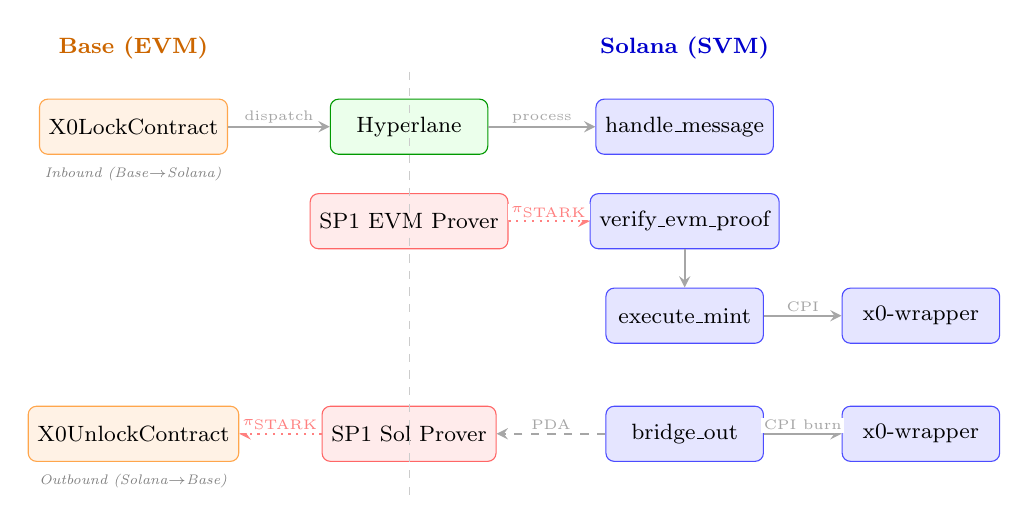
\begin{tikzpicture}[
    node distance=1.2cm and 1.8cm,
    chain/.style={rectangle, rounded corners=3pt, draw=orange!70, fill=orange!10,
        minimum width=2.0cm, minimum height=0.7cm, text centered, font=\footnotesize},
    program/.style={rectangle, rounded corners=3pt, draw=blue!70, fill=blue!10,
        minimum width=2.0cm, minimum height=0.7cm, text centered, font=\footnotesize},
    prover/.style={rectangle, rounded corners=3pt, draw=red!60, fill=red!8,
        minimum width=2.0cm, minimum height=0.7cm, text centered, font=\footnotesize},
    msg/.style={rectangle, rounded corners=3pt, draw=green!60!black, fill=green!8,
        minimum width=2.0cm, minimum height=0.7cm, text centered, font=\footnotesize},
    arrow/.style={->, >=stealth, thick, color=gray!70},
    lbl/.style={font=\tiny, fill=white, inner sep=1pt}
]
    % Title labels
    \node[font=\footnotesize\bfseries, color=orange!80!black] (baselbl) at (-3.5, 1.5) {Base (EVM)};
    \node[font=\footnotesize\bfseries, color=blue!80!black] (sollbl) at (3.5, 1.5) {Solana (SVM)};
    
    % --- Inbound flow (top) ---
    \node[chain] (lock) at (-3.5, 0.5) {X0LockContract};
    \node[msg] (hyp1) at (0, 0.5) {Hyperlane};
    \node[program] (handle) at (3.5, 0.5) {handle\_message};
    
    \node[prover] (evmprover) at (0, -0.7) {SP1 EVM Prover};
    \node[program] (verify) at (3.5, -0.7) {verify\_evm\_proof};
    \node[program] (mint) at (3.5, -1.9) {execute\_mint};
    \node[program] (wrapper1) at (6.5, -1.9) {x0-wrapper};
    
    \draw[arrow] (lock) -- (hyp1) node[lbl, midway, above] {dispatch};
    \draw[arrow] (hyp1) -- (handle) node[lbl, midway, above] {process};
    \draw[arrow, dotted, color=red!50] (evmprover) -- (verify) node[lbl, midway, above] {$\pi_{\text{STARK}}$};
    \draw[arrow] (verify) -- (mint);
    \draw[arrow] (mint) -- (wrapper1) node[lbl, midway, above] {CPI};
    
    % --- Outbound flow (bottom) ---
    \node[program] (bridgeout) at (3.5, -3.4) {bridge\_out};
    \node[program] (wrapper2) at (6.5, -3.4) {x0-wrapper};
    \node[prover] (solprover) at (0, -3.4) {SP1 Sol Prover};
    \node[chain] (unlock) at (-3.5, -3.4) {X0UnlockContract};
    
    \draw[arrow] (bridgeout) -- (wrapper2) node[lbl, midway, above] {CPI burn};
    \draw[arrow, dotted, color=red!50] (solprover) -- (unlock) node[lbl, midway, above] {$\pi_{\text{STARK}}$};
    \draw[arrow, dashed] (bridgeout) -- (solprover) node[lbl, midway, above] {PDA};
    
    % Divider
    \draw[dashed, gray!40] (0, 1.2) -- (0, -4.2);
    
    % Labels
    \node[font=\tiny, color=gray] at (-3.5, -0.1) {\textit{Inbound (Base$\to$Solana)}};
    \node[font=\tiny, color=gray] at (-3.5, -4.0) {\textit{Outbound (Solana$\to$Base)}};
\end{tikzpicture}
\end{center}

\begin{center}
\small\textit{Figure 2: FROSTGATE Bridge Architecture. Orange nodes are EVM contracts. Blue nodes are Solana programs. Red nodes are off-chain SP1 provers.}
\end{center}

\subsection{On-Chain State}

\subsubsection{Bridge Configuration}

The bridge is governed by a singleton PDA seeded by \texttt{["bridge\_config"]}:

\begin{lstlisting}[language=Rust,caption=BridgeConfig State Account]
pub struct BridgeConfig {
    pub admin: Pubkey,             // Multisig administrator
    pub hyperlane_mailbox: Pubkey, // Hyperlane mailbox program
    pub sp1_verifier: Pubkey,      // SP1 verifier program
    pub wrapper_program: Pubkey,   // x0-wrapper for CPI
    pub wrapper_config: Pubkey,    // x0-wrapper config PDA
    pub usdc_mint: Pubkey,         // USDC mint on Solana
    pub wrapper_mint: Pubkey,      // x0-USD mint
    pub bridge_usdc_reserve: Pubkey, // USDC reserve token account
    pub is_paused: bool,
    pub total_bridged_in: u64,     // All-time inflow (USDC micro-units)
    pub total_bridged_out: u64,    // All-time outflow
    pub nonce: u64,                // Monotonic message nonce
    pub daily_inflow_volume: u64,  // Rolling 24h inflow
    pub daily_outflow_volume: u64, // Rolling 24h outflow
    pub allowed_evm_contracts: [[u8; 20]; 10], // Whitelisted EVM contracts
    pub supported_domains: [u32; 10],          // Hyperlane domain IDs
    pub bridge_out_nonce: u64,     // Outbound monotonic nonce
}
\end{lstlisting}

\subsubsection{Bridge Message}

Each inbound Hyperlane message creates a PDA seeded by \texttt{["bridge\_message", message\_id]}:

\begin{lstlisting}[language=Rust,caption=BridgeMessage State Account]
pub struct BridgeMessage {
    pub message_id: [u8; 32],   // SHA-256(origin || sender || body)
    pub origin_domain: u32,     // e.g., 8453 (Base)
    pub sender: [u8; 32],       // EVM address zero-padded to 32 bytes
    pub recipient: Pubkey,      // Solana destination
    pub amount: u64,            // USDC micro-units (6 decimals)
    pub status: BridgeMessageStatus, // Received -> ProofVerified -> Minted
    pub evm_tx_hash: [u8; 32],  // Source transaction hash
    pub nonce: u64,             // Sender nonce for ordering
}
\end{lstlisting}

The message status follows a linear state machine:

\begin{equation}
\texttt{Received} \xrightarrow{\texttt{verify\_evm\_proof}} \texttt{ProofVerified} \xrightarrow{\texttt{execute\_mint}} \texttt{Minted}
\end{equation}

Each transition is irreversible and guarded by status preconditions, ensuring no double-minting.

\subsubsection{EVM Proof Context}

Successful STARK verification creates a PDA seeded by \texttt{["evm\_proof", message\_id]}:

\begin{lstlisting}[language=Rust,caption=EVMProofContext State Account]
pub struct EVMProofContext {
    pub proof_type: EVMProofType,
    pub verified: bool,
    pub verified_at: i64,           // Clock timestamp
    pub block_hash: [u8; 32],       // Proven EVM block hash
    pub block_number: u64,
    pub tx_hash: [u8; 32],          // Proven transaction hash
    pub from: [u8; 20],             // EVM sender
    pub to: [u8; 20],               // EVM contract address
    pub value: u64,
    pub event_logs: Vec<EVMEventLog>, // Extracted receipt logs
    pub message_id: [u8; 32],       // Links to BridgeMessage
}
\end{lstlisting}

\subsubsection{Bridge Out Message}

Each outbound transfer creates a PDA seeded by {\small\texttt{["bridge\_out\_message",\allowbreak{} nonce.to\_le\_bytes()]}}:

\begin{lstlisting}[language=Rust,caption=BridgeOutMessage State Account]
pub struct BridgeOutMessage {
    pub nonce: u64,                // Monotonic from BridgeConfig
    pub solana_sender: Pubkey,     // Burn initiator
    pub evm_recipient: [u8; 20],   // Base destination address
    pub amount: u64,               // USDC micro-units
    pub burn_tx_signature: [u8; 32], // Solana transaction signature
    pub burned_at: i64,            // Burn timestamp
    pub status: BridgeOutStatus,   // Burned -> Unlocked
}
\end{lstlisting}

\subsection{Inbound Protocol (Base $\to$ Solana)}

\subsubsection{Step 1: USDC Lock on Base}

The \texttt{X0LockContract} (Solidity, OpenZeppelin) receives USDC via \texttt{transferFrom}, stores it in the contract, and dispatches a Hyperlane message:

\begin{definition}[Bridge Message Body]
The message body is a tightly-packed 80-byte encoding:
\begin{equation}
\texttt{body} = \texttt{solanaRecipient}_{[32]} \;\|\; \texttt{amount}_{\text{BE}[8]} \;\|\; \texttt{txHash}_{[32]} \;\|\; \texttt{nonce}_{\text{BE}[8]}
\end{equation}
where $\|$ denotes concatenation and subscripts indicate byte lengths. Big-endian encoding is used for all integer fields to match EVM conventions.
\end{definition}

The lock emits a \texttt{Locked} event with indexed parameters for efficient filtering:

\begin{equation}
\texttt{Locked}(\underbrace{\texttt{sender}}_{\text{indexed}}, \;\underbrace{\texttt{solanaRecipient}}_{\text{indexed}}, \;\texttt{amount}, \;\texttt{nonce}, \;\texttt{messageId})
\end{equation}

The event signature is the Keccak-256 hash of the full event declaration:
\begin{equation}
\texttt{topics}[0] = \texttt{keccak256}(\texttt{"Locked(address,bytes32,uint256,uint256,bytes32)"})
\end{equation}

This hash is stored as a protocol constant and used by both the SP1 circuit and the on-chain verifier to locate the deposit event in receipt logs.

\subsubsection{Step 2: Hyperlane Message Delivery}

The Hyperlane protocol relays the message body to Solana, invoking the bridge program's \texttt{handle\_message} instruction. The instruction validates:

\begin{algorithm}
\caption{Inbound Message Reception (\texttt{handle\_message})}
\begin{algorithmic}[1]
\Procedure{HandleMessage}{$\texttt{origin}, \texttt{sender}, \texttt{body}$}
    \State \textbf{require} $\neg\, \texttt{config.is\_paused}$ \Comment{Bridge not paused}
    \State \textbf{require} $\texttt{ValidateProcessAuthority}(\texttt{caller})$ \Comment{Hyperlane PDA}
    \State \textbf{require} $\texttt{origin} \in \texttt{config.supported\_domains}$ \Comment{Known domain}
    \State \textbf{require} $\texttt{sender}[0..12] = \mathbf{0}^{12}$ \Comment{EVM format}
    \State $\texttt{evm\_addr} \gets \texttt{sender}[12..32]$
    \State \textbf{require} $\texttt{evm\_addr} \in \texttt{config.allowed\_evm\_contracts}$ \Comment{Whitelist}
    \State \textbf{require} $|\texttt{body}| = 80$ \Comment{Exact body size}
    \State $(\texttt{recipient}, a, \texttt{tx\_hash}, n) \gets \texttt{decode}(\texttt{body})$
    \State \textbf{require} $a \in [\texttt{MIN\_AMOUNT}, \texttt{MAX\_AMOUNT}]$ \Comment{Bounds check}
    \State \textbf{require} $\texttt{daily\_inflow} + a \leq \texttt{MAX\_DAILY\_INFLOW}$ \Comment{Rate limit}
    \State $\texttt{id} \gets \texttt{SHA256}(\texttt{origin} \;\|\; \texttt{sender} \;\|\; \texttt{body})$
    \State \textbf{create} $\texttt{BridgeMessage}(\texttt{id}, \texttt{origin}, \texttt{sender}, \texttt{recipient}, a)$
\EndProcedure
\end{algorithmic}
\end{algorithm}

\begin{remark}[Hyperlane Process Authority]
The bridge validates the caller by deriving the Hyperlane process authority PDA:
\begin{multline}
\texttt{process\_authority} = \texttt{PDA}_{\texttt{mailbox}}\bigl(\texttt{"hyperlane"} \;\|\; \texttt{"-"} \;\|\;\\
\texttt{"process\_authority"} \;\|\; \texttt{"-"} \;\|\; \texttt{bridge\_id}\bigr)
\end{multline}
This ensures only messages routed through the Hyperlane mailbox can trigger bridge message creation, even if an adversary constructs a valid-looking message body.
\end{remark}

\subsubsection{Step 3: STARK Proof Verification}

After the BridgeMessage is created, an off-chain relayer generates an SP1 STARK proof of the EVM transaction and submits it via \texttt{verify\_evm\_proof}. This instruction:

\begin{enumerate}
    \item Invokes the SP1 verifier program via CPI to verify the STARK proof
    \item Decodes the public inputs: $(h_{\text{block}},\, n_{\text{block}},\, h_{\text{tx}},\, \mathit{from},\, \mathit{to},\, v,\, \mathit{success},\, \mathit{logs})$
    \item Validates $\texttt{success} = \texttt{true}$ (EVM transaction succeeded)
    \item Validates $\texttt{tx\_hash} = \texttt{BridgeMessage.evm\_tx\_hash}$
    \item \textbf{Validates the Locked event} via \texttt{validate\_locked\_event()}
    \item Creates the \texttt{EVMProofContext} PDA and transitions the message to \texttt{ProofVerified}
\end{enumerate}

\begin{definition}[Locked Event Validation]
Given a set of proven event logs $\mathcal{L}$ and a BridgeMessage $M$, the function $\texttt{validate\_locked\_event}(\mathcal{L}, M)$ succeeds if and only if there exists $\ell \in \mathcal{L}$ such that all of the following hold:

\begin{enumerate}
    \item $\ell.\texttt{contract} \in \texttt{config.allowed\_evm\_contracts}$ \hfill (trusted contract)
    \item $\ell.\texttt{topics}[0] = \texttt{LOCKED\_EVENT\_SIGNATURE}$ \hfill (correct event type)
    \item $|\ell.\texttt{topics}| \geq 3$ \hfill (has indexed params)
    \item $\ell.\texttt{topics}[2] = M.\texttt{recipient}$ \hfill (recipient match)
    \item $|\ell.\texttt{data}| \geq 96$ \hfill (three ABI words)
    \item $\texttt{abi.decode}(\ell.\texttt{data}).\texttt{amount} = M.\texttt{amount}$ \hfill (amount match)
    \item $\texttt{abi.decode}(\ell.\texttt{data}).\texttt{nonce} = M.\texttt{nonce}$ \hfill (nonce match)
\end{enumerate}
\end{definition}

\begin{theorem}[Event Validation Soundness]
\label{thm:event-validation}
Under the collision resistance of Keccak-256 and the soundness of the SP1 STARK proof system, no computationally bounded adversary can cause \texttt{validate\_locked\_event} to accept for a BridgeMessage $M$ unless a genuine \texttt{Locked} event with matching recipient, amount, and nonce was emitted by a whitelisted contract in a finalized Base transaction.
\end{theorem}

\begin{proof}
Suppose an adversary $\mathcal{A}$ causes acceptance without a genuine event. Then either:
\begin{enumerate}
    \item $\mathcal{A}$ forged the SP1 proof (contradicts STARK soundness with $\leq 2^{-100}$ forgery probability),
    \item $\mathcal{A}$ found a collision in the event signature (contradicts Keccak-256 collision resistance), or
    \item $\mathcal{A}$ caused a whitelisted contract to emit a \texttt{Locked} event with the adversary's chosen parameters---but this requires calling \texttt{lock()} with matching \texttt{amount} and \texttt{solanaRecipient}, which requires the adversary to actually deposit USDC, making the event genuine.
\end{enumerate}
All cases lead to contradiction. \qed
\end{proof}

\subsubsection{Step 4: Mint Execution}

Once the proof is verified, \texttt{execute\_mint} performs the mint via two CPIs:

\begin{algorithm}
\caption{Mint Execution (\texttt{execute\_mint})}
\begin{algorithmic}[1]
\Procedure{ExecuteMint}{$\texttt{msg}, \texttt{proof\_ctx}$}
    \State \textbf{require} $\texttt{msg.status} = \texttt{ProofVerified}$
    \State \textbf{require} $\texttt{proof\_ctx.is\_fresh}()$ \Comment{Within 600s window}
    \State \textbf{require} $\texttt{bridge\_reserve.amount} \geq \texttt{msg.amount}$
    \State
    \State \textit{// Step 1: Move USDC from bridge reserve to wrapper reserve}
    \State $\texttt{TransferChecked}(\texttt{bridge\_reserve} \to \texttt{wrapper\_reserve}, \texttt{msg.amount})$
    \State
    \State \textit{// Step 2: CPI to x0-wrapper::bridge\_mint}
    \State $\texttt{x0\_wrapper::bridge\_mint}(\texttt{recipient}, \texttt{msg.amount})$
    \State
    \State $\texttt{msg.status} \gets \texttt{Minted}$
    \State $\texttt{config.total\_bridged\_in} \mathrel{+}= \texttt{msg.amount}$
    \State \textbf{if} $\texttt{config.total\_bridged\_in} > \Theta_{\text{in}}$ \textbf{then}
        \State \quad $\texttt{config.is\_paused} \gets \texttt{true}$ \Comment{Circuit breaker}
    \State \textbf{end if}
\EndProcedure
\end{algorithmic}
\end{algorithm}

\begin{remark}[Wrapper Reserve Invariant Preservation]
The two-step CPI sequence preserves the wrapper reserve invariant (Theorem~8.1). Step 1 transfers USDC into the wrapper's reserve account, increasing $R_{\text{USDC}}$. Step 2 calls \texttt{bridge\_mint}, which validates that the bridge program is the authorized caller, then mints x0-USD, increasing $S_{\text{x0-USD}}$ by the same amount. The wrapper's own \texttt{bridge\_mint} handler independently verifies the reserve balance, ensuring $R_{\text{USDC}}(t) \geq S_{\text{x0-USD}}(t)$ holds after every bridge mint.
\end{remark}

\subsection{Outbound Protocol (Solana $\to$ Base)}

\subsubsection{Step 1: Burn on Solana}

The \texttt{initiate\_bridge\_out} instruction validates the outbound request and burns x0-USD:

\begin{algorithm}
\caption{Outbound Bridge Initiation (\texttt{initiate\_bridge\_out})}
\begin{algorithmic}[1]
\Procedure{BridgeOut}{$\texttt{sender}, \texttt{evm\_recipient}_{[20]}, a$}
    \State \textbf{require} $\neg\, \texttt{config.is\_paused}$
    \State \textbf{require} $\texttt{evm\_recipient} \neq \mathbf{0}^{20}$
    \State \textbf{require} $a \in [\texttt{MIN\_AMOUNT}, \texttt{MAX\_AMOUNT}]$
    \State \textbf{require} $\texttt{daily\_outflow} + a \leq \texttt{MAX\_DAILY\_OUTFLOW}$
    \State
    \State \textit{// CPI: burn x0-USD (returns USDC to bridge reserve)}
    \State $\texttt{x0\_wrapper::bridge\_burn}(\texttt{sender}, a)$
    \State
    \State $n \gets \texttt{config.bridge\_out\_nonce}$
    \State $\texttt{config.bridge\_out\_nonce} \mathrel{+}= 1$
    \State \textbf{create} $\texttt{BridgeOutMessage}(n, \texttt{sender}, \texttt{evm\_recipient}, a)$
    \State $\texttt{config.total\_bridged\_out} \mathrel{+}= a$
    \State \textbf{if} $\texttt{config.total\_bridged\_out} > \Theta_{\text{out}}$ \textbf{then}
        \State \quad $\texttt{config.is\_paused} \gets \texttt{true}$ \Comment{Circuit breaker}
    \State \textbf{end if}
\EndProcedure
\end{algorithmic}
\end{algorithm}

The \texttt{bridge\_burn} CPI performs the inverse of \texttt{bridge\_mint}: it burns the sender's x0-USD tokens and transfers the equivalent USDC from the wrapper's reserve back to the bridge's reserve, preserving the wrapper reserve invariant.

\subsubsection{Step 2: Proof Generation and Unlock on Base}

An off-chain relayer observes the \texttt{BridgeOutMessage} PDA, generates an SP1 STARK proof of its existence and validity, and submits the proof to the \texttt{X0UnlockContract} on Base:

\begin{algorithm}
\caption{Outbound Unlock (\texttt{X0UnlockContract.unlock})}
\begin{algorithmic}[1]
\Procedure{Unlock}{$\texttt{proofBytes}, \texttt{publicValues}$}
    \State $(P_{\text{bridge}}, n, \texttt{sender}, r, a, t, h) \gets \texttt{abi.decode}(\texttt{publicValues})$
    \State \textbf{require} $P_{\text{bridge}} = \texttt{BRIDGE\_PROGRAM\_ID}$ \Comment{Correct program}
    \State \textbf{require} $\neg\, \texttt{processedNonces}[n]$ \Comment{Replay protection}
    \State \textbf{require} $a \leq \texttt{maxPerTransaction}$
    \State \textbf{require} $\texttt{dailyVolume} + a \leq \texttt{maxDailyVolume}$
    \State $\texttt{SP1\_VERIFIER.verifyProof}(\texttt{programVKey}, \texttt{publicValues}, \texttt{proofBytes})$
    \State $\texttt{processedNonces}[n] \gets \texttt{true}$
    \State $\texttt{USDC.safeTransfer}(r, a)$
    \State \textbf{emit} $\texttt{BridgeUnlocked}(n, \texttt{sender}, r, a)$
\EndProcedure
\end{algorithmic}
\end{algorithm}

\subsection{SP1 STARK Proof Circuits}

Both proof circuits are implemented as SP1 guest programs that execute inside the SP1 zkVM.\ The zkVM produces a STARK proof that the guest program executed correctly on the claimed inputs, which can be verified on-chain in $\sim$500,000 compute units.

\subsubsection{EVM Proof Circuit (Base $\to$ Solana)}

The EVM proof circuit proves that a specific transaction was included in a finalized Base block and that its receipt contains the expected event logs.

\begin{definition}[EVM Transaction Inclusion Proof]
\label{def:evm-proof}
Let $H_{\text{rlp}}$ denote the RLP-encoded block header, $T_{\text{rlp}}$ the transaction, $R_{\text{rlp}}$ the receipt, and $\pi_T, \pi_R$ the respective MPT proofs. Given witness $w = (H_{\text{rlp}}, T_{\text{rlp}}, R_{\text{rlp}}, \pi_T, \pi_R)$, the circuit proves:
\begin{align}
h_{\text{block}} &= \texttt{keccak256}(H_{\text{rlp}}) \label{eq:block-hash}\\
r_{\text{tx}} &= \texttt{RLP.decode}(H_{\text{rlp}}).\texttt{txRoot} \label{eq:tx-root}\\
r_{\text{rcpt}} &= \texttt{RLP.decode}(H_{\text{rlp}}).\texttt{receiptsRoot} \label{eq:rcpt-root}\\
\texttt{MPT.verify}(r_{\text{tx}},\; k_T,\; T_{\text{rlp}},\; \pi_T) &= \texttt{true} \label{eq:tx-mpt}\\
\texttt{MPT.verify}(r_{\text{rcpt}},\; k_R,\; R_{\text{rlp}},\; \pi_R) &= \texttt{true} \label{eq:rcpt-mpt}\\
R.\texttt{status} &= 1 \label{eq:status}
\end{align}
and outputs public inputs $x = (h_{\text{block}},\, n_{\text{block}},\, h_{\text{tx}},\, \textit{from},\, \textit{to},\, v,\, \textit{success},\, \textit{logs})$.
\end{definition}

The Merkle Patricia Trie (MPT) proofs anchor the transaction and receipt to the block header's state roots. Since the block hash is a public input committed to by the proof, the verifier on Solana can cross-reference it with a known finalized block hash.

\begin{lstlisting}[language=Rust,caption=EVM Proof Public Inputs (sp1-evm-prover)]
pub struct EVMProofPublicInputs {
    pub block_hash: [u8; 32],
    pub block_number: u64,
    pub tx_hash: [u8; 32],
    pub from: [u8; 20],
    pub to: [u8; 20],
    pub value: u64,
    pub success: bool,
    pub event_logs: Vec<EventLog>,
}

pub struct EventLog {
    pub contract_address: [u8; 20],
    pub topics: Vec<[u8; 32]>,
    pub data: Vec<u8>,
}
\end{lstlisting}

\subsubsection{Solana Proof Circuit (Solana $\to$ Base)}

The Solana proof circuit proves that a \texttt{BridgeOutMessage} PDA exists in a confirmed Solana bank state, with the correct owner and data contents.

\begin{definition}[Solana Account Inclusion Proof]
\label{def:sol-proof}
Let $D$ denote the account data, $\pi_M$ the Merkle proof, $B$ the bank hash components, and $V$ the set of validator votes. Given witness $w = (D, \pi_M, B, V)$, the circuit proves:
\begin{align}
(n, s_{\text{addr}}, r, a, t, s) &= \texttt{parse}(D) \label{eq:parse}\\
s &= \texttt{Burned} \label{eq:burned-status}\\
\texttt{owner}(D) &= P_{\text{bridge}} \label{eq:owner}\\
h_{\text{acct}} &= \texttt{SHA256}(D) \label{eq:acct-hash}\\
\texttt{Merkle}_{16}(h_{\text{acct}},\, \pi_M,\, \delta_{\text{hash}}) &= \texttt{true} \label{eq:merkle16}\\
h_{\text{bank}} &= \texttt{SHA256}(h_{\text{parent}} \| \delta_{\text{hash}} \| \sigma_c \| h_{\text{blk}}) \label{eq:bank-hash}\\
\sum_{\substack{v \in V :\\\texttt{Ed25519}(v.\mathit{pk},\, h_{\text{bank}},\, v.\sigma)}} v.\mathit{stake} &\geq \tfrac{2}{3} {\textstyle\sum_{v \in V}} v.\mathit{stake} \label{eq:quorum}
\end{align}
and outputs $x = \texttt{abi.encode}(P_{\text{bridge}},\, n,\, s_{\text{addr}},\, r,\, a,\, t,\, h_{\text{acct}})$.
\end{definition}

\begin{remark}[Fanout-16 Merkle Trees]
Solana's accounts delta hash uses a fanout-16 Merkle tree rather than a binary tree. Each internal node hashes up to 16 children, reducing tree depth to $\log_{16} N$. The circuit verifies inclusion using this wider branching factor, with $\texttt{MERKLE\_FANOUT} = 16$ as a protocol constant.
\end{remark}

\begin{remark}[Validator Quorum Verification]
The circuit verifies that validators representing at least $\frac{2}{3}$ of the epoch's total stake have signed the bank hash via Ed25519 signatures. This mirrors Solana's Tower BFT consensus, ensuring the proven state is finalized.
\end{remark}

\begin{lstlisting}[language=Rust,caption=Solana Proof Public Inputs (sp1-solana-prover)]
pub struct SolanaProofPublicInputs {
    pub bridge_program_id: [u8; 32],
    pub nonce: u64,
    pub solana_sender: [u8; 32],
    pub evm_recipient: [u8; 20],
    pub amount: u64,
    pub burn_timestamp: i64,
    pub account_hash: [u8; 32],
}

impl SolanaProofPublicInputs {
    /// ABI-encodes to 7x32-byte words for EVM verification
    pub fn abi_encode(&self) -> Vec<u8> { /* 224 bytes */ }
}
\end{lstlisting}

\subsection{Rate Limiting and Circuit Breakers}

FROSTGATE implements defense-in-depth rate limiting on both chains.

\subsubsection{Per-Transaction Bounds}

All transfer amounts are bounded:
\begin{equation}
\texttt{MIN\_BRIDGE\_AMOUNT} = 10 \times 10^6 \leq a \leq 100{,}000 \times 10^6 = \texttt{MAX\_BRIDGE\_AMOUNT\_PER\_TX}
\end{equation}
corresponding to \$10--\$100{,}000 USDC per transaction.

\subsubsection{Daily Rolling Window}

Both inflow and outflow are subject to 24-hour rolling limits:
\begin{equation}
\sum_{\{i \,:\, t_i > t - 86400\}} a_i \leq \Phi_{\max} = 5{,}000{,}000 \times 10^6 \quad (\$5\text{M daily})
\end{equation}

The daily counters reset automatically when $t_{\text{current}} - t_{\text{last\_reset}} \geq 86{,}400$ seconds.

\subsubsection{Circuit Breakers}

Cumulative volume triggers an automatic pause:

\begin{equation}
\texttt{total\_bridged\_in} > \Theta_{\text{in}} = 10^{14} \implies \texttt{is\_paused} \gets \texttt{true}
\end{equation}

The threshold $\Theta_{\text{in}} = \Theta_{\text{out}} = 100{,}000{,}000 \times 10^6$ (\$100M) provides a hard upper bound on cumulative bridge exposure. Once triggered, only the admin can unpause after investigation.

\begin{theorem}[Bounded Bridge Exposure]
For all execution traces, the maximum USDC at risk in the bridge at any time is bounded by:
\begin{equation}
\texttt{exposure}(t) \leq \min\left(\Theta_{\text{in}}, \; \Phi_{\max} \cdot \left\lceil \frac{t - t_0}{86400} \right\rceil\right)
\end{equation}
where $t_0$ is the bridge deployment timestamp.
\end{theorem}

\begin{proof}
The daily inflow cap ensures no more than $\Phi_{\max}$ enters per 24-hour window. The circuit breaker provides an absolute ceiling of $\Theta_{\text{in}}$. Since locked USDC on Base can only be unlocked via a valid outbound proof, the exposure is bounded by the lesser of the cumulative cap and the sum of daily windows. \qed
\end{proof}

\subsection{Proof Freshness}

To prevent indefinite replay of verified proofs, proof contexts enforce a temporal validity window:

\begin{definition}[Bridge Proof Freshness]
An \texttt{EVMProofContext} $C$ is \emph{fresh} at time $t$ if and only if:
\begin{equation}
t - C.\texttt{verified\_at} < \Delta_{\text{bridge}} = 600 \text{ seconds}
\end{equation}
\end{definition}

The 10-minute window accounts for Hyperlane relay latency ($\sim$2--3 minutes), SP1 proving time ($\sim$1 minute), and transaction submission buffer. The window is deliberately larger than the ZK verifier's 300-second window (Section~9) to accommodate cross-chain timing uncertainty.

\subsection{EVM Contracts}

Both Solidity contracts inherit OpenZeppelin's \texttt{Ownable}, \texttt{Pausable}, and \texttt{ReentrancyGuard}, providing:

\begin{itemize}
    \item \textbf{Pausability}: Owner can halt all lock/unlock operations in an emergency.
    \item \textbf{Reentrancy protection}: Guards against callback-based exploits during USDC transfers.
    \item \textbf{Rate limiting}: Independent daily volume caps and per-transaction limits on both contracts.
    \item \textbf{Admin recovery}: Timelocked \texttt{adminUnlock} on the lock contract allows fund recovery if the Solana-side flow permanently fails.
\end{itemize}

\subsubsection{X0LockContract}

The lock contract manages inbound flow (Base $\to$ Solana):

\begin{enumerate}
    \item Receives USDC via \texttt{SafeERC20.safeTransferFrom}
    \item Validates amount bounds and daily rate limits
    \item Dispatches the 80-byte message body via Hyperlane's \texttt{IMailbox.dispatch}
    \item Emits the \texttt{Locked} event with the sender, recipient, amount, nonce, and Hyperlane message ID
    \item Increments the per-user nonce for replay ordering
\end{enumerate}

\subsubsection{X0UnlockContract}

The unlock contract manages outbound flow (Solana $\to$ Base):

\begin{enumerate}
    \item Receives an SP1 proof and ABI-encoded public values
    \item Verifies the proof via \texttt{ISP1Verifier.verifyProof(vkey, values, proof)}
    \item Validates the bridge program ID matches the expected Solana program
    \item Checks replay protection via the \texttt{processedNonces} mapping
    \item Transfers USDC to the EVM recipient via \texttt{SafeERC20.safeTransfer}
\end{enumerate}

\subsection{Administrative Controls}

FROSTGATE administrative operations are subject to a 48-hour timelock, matching the x0-wrapper governance model (Section~8):

\begin{enumerate}
    \item \texttt{schedule\_admin\_action}: Creates a \texttt{BridgeAdminAction} PDA with a monotonic nonce and records the action type (e.g., add/remove EVM contract, add/remove domain, change trusted program addresses).
    \item \texttt{execute\_admin\_action}: Executes after $\texttt{current\_time} - \texttt{scheduled\_at} \geq 172{,}800$ seconds. Validates the action nonce, type, and that the action has not been cancelled.
    \item \texttt{cancel\_admin\_action}: Allows the admin to abort a scheduled action before execution.
\end{enumerate}

This timelock gives users and monitoring systems 48 hours to detect and respond to potentially malicious configuration changes (e.g., adding an attacker-controlled EVM contract to the whitelist).

\subsection{Security Analysis}

\subsubsection{Threat Model}

We extend the base protocol's threat model (Section~10) with bridge-specific adversaries:

\begin{enumerate}
    \item \textbf{Proof Forgery}: Adversary attempts to fabricate an SP1 proof for a nonexistent deposit.
    \item \textbf{Amount Inflation}: Adversary deposits $a$ but attempts to mint $a' > a$ on the destination chain.
    \item \textbf{Recipient Redirection}: Adversary deposits for recipient $r$ but attempts to mint for $r' \neq r$.
    \item \textbf{Replay Attack}: Adversary attempts to reuse a valid proof to mint twice.
    \item \textbf{Hyperlane Compromise}: Adversary controls the Hyperlane relayer and crafts arbitrary messages.
    \item \textbf{EVM Contract Impersonation}: Adversary deploys a malicious contract that emits fake \texttt{Locked} events.
\end{enumerate}

\subsubsection{Mitigations}

\begin{table}[ht!]
\centering
\begin{tabular}{|l|l|}
\hline
\textbf{Attack Vector} & \textbf{Mitigation} \\
\hline
Proof Forgery & SP1 STARK soundness ($\leq 2^{-100}$) \\
Amount Inflation & Event amount validated against BridgeMessage \\
Recipient Redirect & Event recipient validated against BridgeMessage \\
Replay (inbound) & BridgeMessage PDA uniqueness + status machine \\
Replay (outbound) & \texttt{processedNonces} mapping on EVM \\
Hyperlane Compromise & SP1 proof required \emph{in addition} to Hyperlane message \\
Contract Impersonation & Event contract address checked against whitelist \\
\hline
\end{tabular}
\caption{FROSTGATE Attack Vectors and Mitigations}
\end{table}

\begin{theorem}[FROSTGATE Soundness]
\label{thm:frostgate-soundness}
Under the soundness of the SP1 STARK proof system, the collision resistance of SHA-256 and Keccak-256, and the unforgeability of Ed25519 signatures, FROSTGATE is a sound cross-chain bridge (Definition~14.2).
\end{theorem}

\begin{proof}
We show that no minting can occur without a corresponding genuine deposit.

For \emph{inbound} transfers (Base $\to$ Solana):
\begin{enumerate}
    \item \texttt{execute\_mint} requires $\texttt{msg.status} = \texttt{ProofVerified}$.
    \item The \texttt{ProofVerified} status is only set by \texttt{verify\_evm\_proof}, which validates an SP1 STARK proof.
    \item The STARK proof commits to a block hash, transaction hash, and event logs (Definition~\ref{def:evm-proof}).
    \item \texttt{validate\_locked\_event} (Theorem~\ref{thm:event-validation}) ensures the proven event logs contain a genuine \texttt{Locked} event with matching amount, recipient, and nonce from a whitelisted contract.
    \item Therefore, minting requires a valid EVM transaction that deposited the exact amount for the exact recipient.
\end{enumerate}

For \emph{outbound} transfers (Solana $\to$ Base):
\begin{enumerate}
    \item \texttt{X0UnlockContract.unlock} requires a valid SP1 proof of a \texttt{BridgeOutMessage} PDA.
    \item The STARK proof commits to the account hash, nonce, amount, and recipient (Definition~\ref{def:sol-proof}).
    \item Validator quorum verification (Equation~\ref{eq:quorum}) ensures the proven state is finalized under Solana's Tower BFT consensus.
    \item The \texttt{processedNonces} mapping prevents replay.
    \item Therefore, unlocking requires a genuine burn transaction on Solana with finalized consensus. \qed
\end{enumerate}
\end{proof}

\begin{theorem}[FROSTGATE Completeness]
FROSTGATE is a complete cross-chain bridge (Definition~14.3), given liveness of the Hyperlane relayer (inbound) and the SP1 prover operator (both directions).
\end{theorem}

\begin{proof}
For any valid \texttt{Lock} on Base: (1) the Hyperlane relayer delivers the message, creating a \texttt{BridgeMessage} PDA; (2) the SP1 prover generates a valid proof of the EVM transaction; (3) the \texttt{verify\_evm\_proof} instruction verifies the proof and transitions the message to \texttt{ProofVerified}; (4) the \texttt{execute\_mint} instruction mints x0-USD. Each step is deterministic given valid inputs. The only liveness assumptions are on the relayer and prover, which are permissionless roles. \qed
\end{proof}

\begin{theorem}[Reserve Invariant Under Bridge Operations]
For all execution traces involving bridge mint and burn operations:
\begin{equation}
\forall t: R_{\text{USDC}}(t) \geq S_{\text{x0-USD}}(t)
\end{equation}
\end{theorem}

\begin{proof}
Bridge mint: \texttt{execute\_mint} first transfers $a$ USDC from the bridge reserve to the wrapper reserve ($R_{\text{USDC}} \mathrel{+}= a$), then calls \texttt{bridge\_mint} to mint $a$ x0-USD ($S_{\text{x0-USD}} \mathrel{+}= a$). The wrapper's \texttt{bridge\_mint} handler independently verifies $R_{\text{USDC}} \geq S_{\text{x0-USD}}$ before minting.

Bridge burn: \texttt{bridge\_burn} burns $a$ x0-USD ($S_{\text{x0-USD}} \mathrel{-}= a$) and transfers $a$ USDC from the wrapper reserve to the bridge reserve ($R_{\text{USDC}} \mathrel{-}= a$). The decrement is symmetric.

In both cases the invariant is preserved by the wrapper's own validation (Theorem~8.1). \qed
\end{proof}

\section{Future Work}

\subsection{Extended Zero-Knowledge Applications}

With the foundational ZK verification infrastructure now deployed (Section~9), several extensions become feasible:
\begin{itemize}
    \item \textbf{Private spend limit verification}: Prove that a transfer is within policy limits without revealing the daily limit or cumulative spend, using range proofs composed with the existing Groth16 circuits
    \item \textbf{Proof of reputation threshold}: Prove $S \geq \theta$ for a reputation score $S$ and threshold $\theta$ without revealing the exact score, enabling privacy-preserving agent discovery
    \item \textbf{Confidential escrow amounts}: Extend the escrow state machine to operate on encrypted amounts, using ZK proofs to verify state transitions without revealing the escrowed value
    \item \textbf{Recursive proof composition}: Batch multiple proof verifications into a single on-chain instruction using recursive SNARKs, reducing per-transaction compute costs
\end{itemize}

\subsection{Cross-Chain Extension}

With FROSTGATE operational on Base\,$\longleftrightarrow$\,Solana (Section~14), the architecture generalizes to additional EVM chains:
\begin{itemize}
    \item \textbf{Multi-chain deployment}: Deploy \texttt{X0LockContract} and \texttt{X0UnlockContract} instances on Ethereum mainnet, Arbitrum, Optimism, and other EVM chains, each with its own Hyperlane domain ID registered in BridgeConfig
    \item \textbf{Non-EVM chains}: Extend the SP1 proof model to verify state inclusion on non-EVM chains (e.g., Cosmos via IBC, Aptos via Move proofs), enabling a unified cross-chain payment mesh
    \item \textbf{Unified reputation across chains}: Anchor reputation scores to Solana as the settlement layer, with bridge-proven attestations propagating trust scores cross-chain
    \item \textbf{Cross-chain escrow settlement}: Compose FROSTGATE with the escrow protocol (Section~5) to enable trustless cross-chain escrow with atomic settlement guarantees
\end{itemize}

\subsection{Machine Learning Integration}

\begin{itemize}
    \item Anomaly detection for suspicious agent behavior using on-chain transaction patterns
    \item Dynamic reputation weighting via learned feature importance
    \item Predictive escrow dispute resolution using historical outcome data
\end{itemize}

\subsection{Governance}

\begin{itemize}
    \item DAO for protocol parameter updates (fee rates, timelock durations)
    \item Community-driven arbiter selection and staking
    \item Fee redistribution to token holders and active arbiters
\end{itemize}

\section{Conclusion}

We have presented x0, a comprehensive payment infrastructure for autonomous agents. The protocol's key innovations include:

\begin{enumerate}
    \item \textbf{Transfer Hook Policy Enforcement}: Programmable spending limits enforced cryptographically on every transaction
    \item \textbf{HTTP 402 Protocol}: Standardized payment negotiation for agent-to-agent commerce
    \item \textbf{Conditional Escrow}: Trustless high-value transactions with dispute resolution
    \item \textbf{Temporal Reputation}: On-chain trust scores with decay to prevent stale reputations
    \item \textbf{USDC Wrapper}: Stable payments with cryptographic reserve invariants
    \item \textbf{Human-in-the-Loop}: Fallback mechanism for exceptional cases
    \item \textbf{Zero-Knowledge Verification}: On-chain Groth16 proof verification enabling confidential transfers with provable correctness
    \item \textbf{FROSTGATE Bridge}: Trustless bidirectional Base\,$\longleftrightarrow$\,Solana bridging using SP1 STARK proofs and Hyperlane message passing, with event-level validation, rate limiting, and circuit breakers---eliminating all off-chain trust assumptions from cross-chain agent payments
\end{enumerate}

The protocol has been deployed on Solana devnet and is undergoing security audits. We invite the community to review the codebase at \texttt{github.com/x0-protocol} and provide feedback.

The future of AI agent commerce requires infrastructure that is:
\begin{itemize}
    \item \textbf{Fast}: Sub-second transaction finality
    \item \textbf{Cheap}: Sub-cent transaction costs
    \item \textbf{Programmable}: Enforcing complex spending rules
    \item \textbf{Trustless}: No centralized intermediaries
    \item \textbf{Safe}: Bounded downside risk
\end{itemize}

x0 achieves these properties through careful cryptographic design and integration with Solana's high-performance blockchain.

\section*{Acknowledgments}

We thank the Solana Foundation for technical support, the Anchor framework team for excellent developer tooling, and the broader Solana community for feedback during development. Special thanks to the auditors at OtterSec and Trail of Bits for security reviews.

\begin{thebibliography}{99}

\bibitem{bitcoin}
Nakamoto, S. (2008). Bitcoin: A Peer-to-Peer Electronic Cash System.

\bibitem{ethereum}
Buterin, V. (2014). Ethereum: A Next-Generation Smart Contract and Decentralized Application Platform.

\bibitem{solana}
Yakovenko, A. (2018). Solana: A new architecture for a high performance blockchain.

\bibitem{lightning}
Poon, J., \& Dryja, T. (2016). The Bitcoin Lightning Network: Scalable Off-Chain Instant Payments.

\bibitem{raiden}
Raiden Network Team. (2017). Raiden Network: Fast, cheap, scalable token transfers for Ethereum.

\bibitem{token22}
Solana Labs. (2023). Token-2022 Extension Documentation. \url{https://spl.solana.com/token-2022}

\bibitem{elgamal}
ElGamal, T. (1985). A public key cryptosystem and a signature scheme based on discrete logarithms. IEEE Transactions on Information Theory, 31(4), 469-472.

\bibitem{merkle}
Merkle, R. C. (1988). A Digital Signature Based on a Conventional Encryption Function. CRYPTO '87.

\bibitem{bloom}
Bloom, B. H. (1970). Space/time trade-offs in hash coding with allowable errors. Communications of the ACM, 13(7), 422-426.

\bibitem{ed25519}
Bernstein, D. J., et al. (2012). High-speed high-security signatures. Journal of Cryptographic Engineering, 2(2), 77-89.

\bibitem{groth16}
Groth, J. (2016). On the Size of Pairing-Based Non-interactive Arguments. EUROCRYPT 2016, Lecture Notes in Computer Science, vol 9666, pp. 305-326.

\bibitem{ristretto}
Hamburg, M. (2015). Decaf: Eliminating cofactors through point compression. CRYPTO 2015. Extended to Ristretto255 for use with Curve25519.

\bibitem{sp1}
Succinct Labs. (2024). SP1: A performant, open-source zero-knowledge virtual machine. \url{https://docs.succinct.xyz}

\bibitem{hyperlane}
Hyperlane. (2024). Hyperlane: Permissionless Interoperability. \url{https://docs.hyperlane.xyz}

\bibitem{stark}
Ben-Sasson, E., Bentov, I., Horesh, Y., \& Riabzev, M. (2018). Scalable, transparent, and post-quantum secure computational integrity. IACR Cryptology ePrint Archive, 2018, 046.

\bibitem{mpt}
Wood, G. (2014). Ethereum: A Secure Decentralised Generalised Transaction Ledger. Ethereum Yellow Paper, Appendix D: Modified Merkle Patricia Trie.

\end{thebibliography}

\appendix

\section{Error Codes Reference}

Error codes follow a structured numbering scheme where the high byte identifies the program category and the low nibble groups errors by subcategory:

{\scriptsize
\setlength{\tabcolsep}{4pt}
\renewcommand{\arraystretch}{0.9}
\begin{longtable}{|l|l|l|}
\hline
\textbf{Range} & \textbf{Name} & \textbf{Description} \\
\hline
\endfirsthead
\hline
\textbf{Range} & \textbf{Name} & \textbf{Description} \\
\hline
\endhead
\hline
\endfoot
\hline
\multicolumn{3}{|c|}{\textit{x0-guard: Policy Errors (0x1100--0x110F)}} \\
\hline
0x1101 & RecipientNotWhitelisted & Recipient not in whitelist \\
0x1102 & DailyLimitExceeded & Rolling 24h limit exceeded \\
0x1103 & InvalidMerkleProof & Merkle proof verification failed \\
0x1104 & InvalidBloomFilter & Bloom filter misconfigured \\
0x1105 & PolicyNotFound & Agent policy PDA missing \\
0x1106 & UnauthorizedSigner & Unauthorized transaction signer \\
0x1107 & ConfidentialTransferFailed & ZK proof verification failed \\
\hline
\multicolumn{3}{|c|}{\textit{x0-guard: Configuration Errors (0x1110--0x111F)}} \\
\hline
0x1110 & DailyLimitTooHigh & Exceeds maximum daily limit \\
0x1111 & DailyLimitTooLow & Below minimum daily limit \\
0x1112 & InvalidWhitelistConfig & Invalid whitelist configuration \\
0x1118 & DelegationRequired & Agent must be delegate, not owner \\
0x111B & BoundTokenAccountMismatch & Wrong source token account \\
0x111F & MissingZkProof & ZK proof required for confidential transfer \\
\hline
\multicolumn{3}{|c|}{\textit{x0-guard: Transfer Errors (0x1120--0x112F)}} \\
\hline
0x1120 & ZeroTransferAmount & Transfer amount is zero \\
0x1121 & TransferAmountTooHigh & Exceeds per-transaction limit \\
\hline
\multicolumn{3}{|c|}{\textit{x0-guard: Blink Errors (0x1130--0x113F)}} \\
\hline
0x1130 & BlinkRateLimitExceeded & $>$3 blinks per hour \\
0x1131 & BlinkExpired & Blink has expired \\
\hline
\multicolumn{3}{|c|}{\textit{x0-guard: Severity Errors (0x1140--0x114F)}} \\
\hline
0x1140 & PolicyUpdateTooFrequent & Rate-limited policy update \\
0x1141 & SingleTransactionLimitExceeded & Per-tx limit exceeded \\
0x1143 & ExtraMetasAlreadyInitialized & Extra metas re-init blocked \\
0x1144 & UnauthorizedExtraMetasInitializer & Mint authority required \\
\hline
\multicolumn{3}{|c|}{\textit{x0-escrow: State Errors (0x1108--0x1109, 0x1200+)}} \\
\hline
0x1108 & EscrowExpired & Escrow timeout reached \\
0x1109 & InvalidEscrowState & Invalid state transition \\
0x1202 & SameBuyerAndSeller & Buyer and seller must differ \\
0x1204 & ZeroEscrowAmount & Escrow amount is zero \\
\hline
\multicolumn{3}{|c|}{\textit{x0-escrow: Operation Errors (0x1210--0x121F)}} \\
\hline
0x1210 & OnlyBuyerCanFund & Only buyer can fund \\
0x1211 & OnlySellerCanDeliver & Only seller can mark delivered \\
0x1213 & OnlyArbiterCanResolve & Only arbiter can resolve \\
0x1217 & ArbiterResolutionTooEarly & Arbiter must wait for delay \\
\hline
\multicolumn{3}{|c|}{\textit{x0-registry: Entry Errors (0x1300--0x130F)}} \\
\hline
0x1300 & AgentAlreadyRegistered & Agent already registered \\
0x1301 & AgentNotFound & Agent not found \\
0x1303 & EndpointTooLong & Endpoint URL too long \\
0x1304 & TooManyCapabilities & Exceeds max capabilities \\
0x1307 & InsufficientListingFee & Listing fee not met \\
\hline
\multicolumn{3}{|c|}{\textit{x0-reputation: Errors (0x1400--0x140F)}} \\
\hline
0x1400 & ReputationNotFound & Reputation account missing \\
0x1401 & ReputationAlreadyInitialized & Already initialized \\
0x1403 & UnauthorizedReputationUpdate & Unauthorized caller \\
0x1404 & InsufficientTransactions & Too few txns for score \\
\hline
\multicolumn{3}{|c|}{\textit{x0-token: Token Errors (0x1500--0x1515)}} \\
\hline
0x1500 & MintAlreadyInitialized & Mint already initialized \\
0x1503 & ConfidentialTransfersNotEnabled & Confidential not enabled \\
0x1507 & InvalidElGamalPubkey & Invalid ElGamal public key \\
0x1508 & InvalidPubkeyValidityProof & Invalid pubkey proof \\
0x150A & InvalidWithdrawProof & Invalid withdraw proof \\
0x150F & AmountExceedsConfidentialMax & Amount $> 2^{48}-1$ \\
\hline
\multicolumn{3}{|c|}{\textit{x0-wrapper: State/Reserve Errors (0x1600--0x164F)}} \\
\hline
0x1600 & WrapperPaused & Operations are paused \\
0x1610 & InsufficientReserve & Insufficient reserve balance \\
0x1611 & ReserveInvariantViolated & Reserve $<$ supply \\
0x1620 & DepositTooSmall & Below minimum deposit \\
0x1623 & DailyRedemptionLimitExceeded & Daily limit exceeded \\
0x1630 & Unauthorized & Admin required \\
0x1640 & AdminActionNotFound & Action PDA not found \\
0x1643 & TimelockNotExpired & Timelock period pending \\
\hline
\multicolumn{3}{|c|}{\textit{x0-zk-verifier: Proof Errors (0x1700--0x1721)}} \\
\hline
0x1700 & ProofVerificationFailed & ZK proof verification failed \\
0x1701 & InvalidProofData & Invalid proof data format \\
0x1703 & InvalidProofType & Invalid proof type \\
0x1704 & ProofExpired & Proof timestamp too old \\
0x1710 & AmountTooLarge & Amount $> 2^{48}-1$ \\
0x1711 & InvalidElGamalPubkey & Invalid ElGamal public key \\
0x1713 & ProofSizeMismatch & Proof data size mismatch \\
0x1720 & ArithmeticOverflow & Arithmetic overflow \\
\hline
\multicolumn{3}{|c|}{\textit{x0-bridge: Configuration Errors (0x1800--0x1806)}} \\
\hline
0x1800 & BridgeAlreadyInitialized & Bridge already initialized \\
0x1802 & BridgePaused & Bridge operations are paused \\
0x1803 & Unauthorized & Admin required \\
0x1805 & InvalidSP1Verifier & Invalid SP1 verifier program \\
\hline
\multicolumn{3}{|c|}{\textit{x0-bridge: Message Errors (0x1810--0x1819)}} \\
\hline
0x1810 & UnsupportedDomain & Origin domain not supported \\
0x1811 & UnauthorizedSenderContract & Sender contract not in allowed list \\
0x1812 & MessageAlreadyProcessed & Message already processed \\
0x1817 & InvalidProcessAuthority & PDA derivation mismatch \\
0x1818 & InvalidSenderFormat & EVM sender zero-padding check \\
0x1819 & CircuitBreakerTriggered & Bridge volume exceeds threshold \\
\hline
\multicolumn{3}{|c|}{\textit{x0-bridge: Proof Errors (0x1820--0x182D)}} \\
\hline
0x1820 & ProofVerificationFailed & STARK proof verification failed \\
0x1823 & ProofExpired & Proof exceeded validity window \\
0x1826 & DepositEventNotFound & Locked event not in proof logs \\
0x1828 & EventContractMismatch & Event from unauthorized contract \\
0x1829 & EventRecipientMismatch & Event recipient $\neq$ message recipient \\
0x182A & EventAmountMismatch & Event amount $\neq$ message amount \\
0x182B & EventNonceMismatch & Event nonce $\neq$ expected nonce \\
\hline
\multicolumn{3}{|c|}{\textit{x0-bridge: Rate Limiting (0x1830--0x183F)}} \\
\hline
0x1830 & AmountTooSmall & Bridge amount $<$ minimum \\
0x1831 & AmountTooLarge & Bridge amount $>$ per-tx max \\
0x1832 & DailyInflowLimitExceeded & Daily inflow limit exceeded \\
0x1833 & InsufficientBridgeReserve & Insufficient reserve for minting \\
\hline
\multicolumn{3}{|c|}{\textit{x0-bridge: Outbound Errors (0x1870--0x1876)}} \\
\hline
0x1870 & BridgeOutPaused & Outbound operations paused \\
0x1873 & DailyOutflowLimitExceeded & Daily outflow limit exceeded \\
0x1874 & OutboundCircuitBreakerTriggered & Outbound circuit breaker \\
0x1875 & InvalidEvmRecipient & Invalid EVM recipient address \\
\hline
\caption{Protocol Error Codes (representative subset; 8 enums, 90+ total codes). Full reference in source: \texttt{x0-common/src/error.rs}}
\end{longtable}
}

\section{Program Addresses}

\begin{table}[ht!]
\centering
\begin{tabular}{|l|l|}
\hline
\textbf{Program} & \textbf{Devnet Address} \\
\hline
x0-guard & \texttt{2uYGW3fQUGfhrwVbkupdasXBpRPfGYBGTLUdaPTXU9vP} \\
x0-token & \texttt{EHHTCSyGkmnsBhGsvCmLzKgcSxtsN31ScrfiwcCbjHci} \\
x0-escrow & \texttt{AhaDyVm8LBxpUwFdArA37LnHvNx6cNWe3KAiy8zGqhHF} \\
x0-registry & \texttt{Bebty49EPhFoANKDw7TqLQ2bX61ackNav5iNkj36eVJo} \\
x0-reputation & \texttt{FfzkTWRGAJQPDePbujZdEhKHqC1UpqvDrpv4TEiWpx6y} \\
x0-wrapper & \texttt{EomiXBbg94Smu4ipDoJtuguazcd1KjLFDFJt2fCabvJ8} \\
x0-zk-verifier & \texttt{zQWSrznKgcK8aHA4ry7xbSCdP36FqgUHj766YM3pwre} \\
x0-bridge & \texttt{4FuyKfQysHxcTeNJtz5rBzzS8kmjn2DdkgXH1Q7edXa7} \\
\hline
\end{tabular}
\caption{Deployed Program Addresses}
\end{table}

\section{Mathematical Notation}

\begin{table}[ht!]
\centering
\begin{tabular}{|l|l|}
\hline
\textbf{Symbol} & \textbf{Meaning} \\
\hline
$H$ & Cryptographic hash function (SHA-256) \\
$sk, pk$ & Secret key, public key \\
$\sigma$ & Digital signature \\
$L$ & Daily spending limit \\
$x_i$ & Transaction amount at index $i$ \\
$t_i$ & Transaction timestamp at index $i$ \\
$R$ & Recipient address \\
$W$ & Whitelist set \\
$n$ & Number of transactions \\
$m$ & Number of whitelist entries \\
$k$ & Number of hash functions (Bloom) \\
$S$ & Reputation score \\
$\rho$ & Reserve ratio \\
$R_{\text{USDC}}$ & USDC reserve balance \\
$S_{\text{x0-USD}}$ & x0-USD supply \\
$G, H$ & Ristretto255 generators \\
$P$ & ElGamal public key ($P = s \cdot G$) \\
$s$ & ElGamal secret scalar \\
$\pi$ & Zero-knowledge proof ($\pi = (A, B, C)$ for Groth16) \\
$\Delta_{\text{proof}}$ & Proof freshness window (300 seconds) \\
$\Delta_{\text{bridge}}$ & Bridge proof freshness window (600 seconds) \\
$\Theta_{\text{in}}, \Theta_{\text{out}}$ & Circuit breaker thresholds (\$100M) \\
$\Phi_{\max}$ & Maximum daily bridge volume (\$5M) \\
$\delta_{\text{hash}}$ & Solana accounts delta hash \\
$h_{\text{bank}}$ & Solana bank hash \\
\hline
\end{tabular}
\caption{Mathematical Notation Reference}
\end{table}

\section{SDK Integration Guide}

\subsection{Installation}

The x0 TypeScript SDK is available via npm:

\begin{lstlisting}[language=bash,caption=SDK Installation]
npm install @x0-protocol/sdk
# or
yarn add @x0-protocol/sdk
\end{lstlisting}

\subsection{Quick Start}

\begin{lstlisting}[language=JavaScript,caption=Basic SDK Usage]
import { 
  X0Client, 
  EscrowClient, 
  ReputationClient,
  createPaymentRequest,
  verifyPaymentProof 
} from '@x0-protocol/sdk';
import { Connection, Keypair } from '@solana/web3.js';

// Initialize connection
const connection = new Connection('https://api.devnet.solana.com');
const wallet = Keypair.generate(); // or load from file

// Create escrow
const escrow = new EscrowClient(connection);
const { escrowPda, tx } = await escrow.buildCreateEscrowInstruction({
  buyer: wallet.publicKey,
  seller: sellerPubkey,
  amount: 1_000_000, // 1 USDC (6 decimals)
  memo: 'API service payment',
  timeoutSeconds: 86400, // 24 hours
});

// x402 payment flow (service side)
const paymentRequest = createPaymentRequest({
  recipient: servicePubkey,
  amount: '1000000',
  resource: '/api/v1/generate',
  network: 'solana-devnet',
});

// Verify payment (service side)
const isValid = await verifyPaymentProof(connection, proof, {
  expectedRecipient: servicePubkey,
  expectedAmount: 1_000_000,
  toleranceSeconds: 300,
});
\end{lstlisting}

\subsection{SDK Modules}

\begin{table}[ht!]
\centering
\begin{tabular}{|l|l|}
\hline
\textbf{Module} & \textbf{Purpose} \\
\hline
\texttt{EscrowClient} & Create, fund, release, dispute escrows \\
\texttt{ReputationClient} & Query and update agent reputation \\
\texttt{RegistryClient} & Register agents, discover services \\
\texttt{GuardClient} & Manage spending policies \\
\texttt{WrapperClient} & Wrap/unwrap USDC to x0-USD \\
\texttt{ConfidentialClient} & Confidential transfer proof generation via WASM \\
\texttt{ZkVerifierClient} & On-chain ZK proof verification \\
\texttt{x402} & HTTP 402 payment request/proof utilities \\
\texttt{blink} & Generate Solana Actions for human approval \\
\texttt{BridgeClient} & Cross-chain bridge operations (lock, verify, mint, bridge-out) \\
\hline
\end{tabular}
\caption{SDK Module Overview}
\end{table}

\subsection{Resources}

\begin{itemize}
    \item \textbf{npm}: \texttt{https://npmjs.com/package/@x0-protocol/sdk}
    \item \textbf{GitHub}: \texttt{https://github.com/0xtnxl/x0/sdk}
    \item \textbf{API Docs}: \texttt{https://docs.x0protocol.dev/sdk}
    \item \textbf{Examples}: \texttt{https://github.com/0xtnxl/x0/examples}
\end{itemize}

\subsection{Confidential Transfer Architecture}

For the complete treatment of the zero-knowledge proof system---including cryptographic foundations, proof types, the \texttt{ProofContext} state account, and the end-to-end verification flow---see Section~9. The SDK's \texttt{ConfidentialClient} module wraps the WASM-compiled \texttt{x0-zk-proofs} crate to provide transparent proof generation:

\begin{lstlisting}[language=JavaScript,caption=Confidential Transfer ZK Proof Generation]
import { ConfidentialClient } from '@x0-protocol/sdk';

const confidentialClient = new ConfidentialClient(connection, wallet);

// Proof generation via WASM (x0-zk-proofs):
// - PubkeyValidityProof: Proves ElGamal key validity (64 bytes)
// - WithdrawProof: Proves withdrawal against encrypted balance (160 bytes)
// - ZeroBalanceProof: Proves zero balance for account closure (96 bytes)
// On-chain verification via x0-zk-verifier creates ProofContext PDAs
// that Token-2022 references during confidential transfer execution.
\end{lstlisting}

\end{document}